%%%%%%%%%%%%%%%%%%%%%%%%%%%%%%%%%%%%%%%%%%%%%%%%%%%%%%%%%%%%%%%%%%%%%%%%%%%
%% Rulebook RoboCup Logistics League Sponsored by Festo
%% 2014 Competitions
%%%%%%%%%%%%%%%%%%%%%%%%%%%%%%%%%%%%%%%%%%%%%%%%%%%%%%%%%%%%%%%%%%%%%%%%%%%

\documentclass[12pt,twoside]{article}

\usepackage[a4paper]{anysize}
\marginsize{2.5cm}{2cm}{2cm}{2cm}

\setlength{\marginparwidth}{1cm}
%\usepackage{fourier}
%\newcommand\rulechange[1]{\begin{shaded}#1\end{shaded}\marginpar{\LARGE\danger}}

%% MACROS %%%%%%%%%%%%%%%%%%%

% does not work for me, gives:
%! Undefined control sequence.
%\@ympar ...lobal \setbox \@currbox \copy \@marbox 
%                                                  \@xympar 
%\newenvironment{rulechange}{%
%  \def\FrameCommand{\fboxsep=\FrameSep \colorbox{shadecolor}}%
%  \marginpar{\vspace*{2em}\LARGE\danger} \MakeFramed  {\FrameRestore}}%
% { \endMakeFramed}
\newenvironment{rulechange}{}{}

\usepackage[binary-units=true]{siunitx}

%\usepackage{framed,xcolor}
%\colorlet{shadecolor}{gray!25}
%\textregistered
\newcommand{\Robotino}{Robotino}
\newcolumntype{R}{>{\raggedleft\arraybackslash}X}
\newcolumntype{C}{>{\centering\arraybackslash}X}

\newsavebox{\myt}
\newcommand{\mytable}[1]{\savebox{\myt}{#1}\tikz\node[fill=gray!25!white]{\usebox{\myt}};}

\newcommand{\refsec}[1]{Section~\ref{#1}}
\newcommand{\reffig}[1]{Figure~\ref{#1}}
\newcommand{\refdef}[1]{Definition~\ref{#1}}
%\newcommand{\reflst}[1]{Listing~\ref{#1}}
\newcommand{\reflst}[1]{Figure~\ref{#1}}

\usepackage{floatrow}
\newfloatcommand{capbtabbox}{table}[][\FBwidth]


%% GRAPHICSX %%%%%%%%%%%%%%%%%%%
\usepackage[pdftex]{graphicx}
\graphicspath{{figures/}}
\DeclareGraphicsExtensions{.pdf,.jpeg,.png,.JPG,.jpg}

%% TIKZ %%%%%%%%%%%%%%%%%%%
\usepackage{tikz}
\usetikzlibrary{arrows,shadows}
\usetikzlibrary{calc,positioning}
\usetikzlibrary{snakes,shapes}
\usetikzlibrary{shapes.callouts}

%% HYPERREF %%%%%%%%%%%%%%%%%%%
\usepackage{hyperref}
\hypersetup{
  pdftitle      = {The Logistics League 2014 sponsored by Festo Rulebook for 2014},
  pdfauthor     = {LLSF TC},
  pdfkeywords   = {LLSF, Rulebook},
  pdfsubject    = {},
  %pdfpagemode   = {UseOutlines},        % PageWdth, FullScreen, None ...
  hidelinks    = true,          % true colored links, false colored boxes
%  linkcolor     = black,
%  citecolor     = black,
%  filecolor     = black,
%  urlcolor      = black,
%  backref       = false,
%  pagecolor     = black,         % link to other document pages
%  linktocpage,                  % linked page numbers instead of titles
%  menucolor   = blue,           % Acrobat menu item
%  pdfnewwindow= true,                %
%  pdfborder   = {0 0 0},             %
%  bookmarksopen=true,                %
%  bookmarksnumbered=true,            %
%  pdfcreator   = {pdflatex},
%  pdfproducer  = {latex-pdftex}
}

%% SVN-MULTI %%%%%%%%%%%%%%%%%%%
%\usepackage{svn-multi}

%% TODONOTES %%%%%%%%%%%%%%%%%%%
\usepackage{todonotes}

%% TIMES  %%%%%%%%%%%%%%%%%%%
\usepackage{times}

%% TABLES %%%%%%%%%%%%%%%%%%%
\usepackage{tabularx}
\usepackage{multicol}
\usepackage{multirow}
\usepackage{calc}
\usepackage{float}
\restylefloat{table}

\usepackage[TABBOTCAP]{subfigure}
%% INPUTENC %%%%%%%%%%%%%%%%%%%
\usepackage{wasysym}
\usepackage[utf8]{inputenc}
%%%%%%%%%%%%%%%%%%%%%%%%%%%%%%%%%%%%%%%%%%%%%%%%%%%%%%%%%%%%%%%%%%%%%%%%%%%%%
%%% Ruebook RoboCup Logistics League Sponsored by Festo 
%%% Draft for 2013 Competition
%%%%%%%%%%%%%%%%%%%%%%%%%%%%%%%%%%%%%%%%%%%%%%%%%%%%%%%%%%%%%%%%%%%%%%%%%%%%%


\newcommand{\s}[1]{\ensuremath{S_{#1}}}
\newcommand{\p}[1]{\ensuremath{P_{#1}}}
\newcommand{\m}[1]{\ensuremath{M_{#1}}}
\newcommand{\T}[1]{\ensuremath{T_{#1}}}
\newcommand{\dg}[1]{\ensuremath{DG_{#1}}}
\newcommand{\TAG}[1]{\texttt{#1}}


\usepackage[style=numeric,backend=bibtex,maxbibnames=10]{biblatex}
\addbibresource{rulebook2014}


\begin{document}

%%%%%%%%%%%%%%%%%%%%%%%%%%%%%%%%%%%%%%%%%%%%%%%%%%%%%%%%%%%%%%%%%%%%%%%%%%%%%
%%% Titlepage
\hypersetup{pageanchor=false}
\pagenumbering{roman}


\begin{titlepage}
  \vspace*{5cm}
  \begin{center}
    \begin{LARGE}
      
      {\bf RoboCup Logistics League sponsored by Festo}\\[2ex]
      {\Large Rules and Regulations 2014}\\[4ex]
    \end{LARGE}
    \hrule
    
    {\LARGE\vspace*{4ex}}
    \begin{Large}
      The Technical Committee 2012--2014\\[6ex]
    \end{Large}
    \begin{tabular}{lll}
    \emph{Christian Deppe}&Daniel Ewert&\emph{Nils Harder}\\
    \emph{S\"oren Jentzsch}&\emph{Nicolas Meier}&\emph{Tim Niemueller}\\
      Sebastian Reuter&\emph{Alain Rohr}&\emph{Wataru Uemura}\\
    \end{tabular}
    \vfill
    Revision Date: January 30$^\mathrm{th}$ 2014
  \end{center}
\end{titlepage}
\thispagestyle{empty}
\pagebreak
\clearpage

%%%%%%%%%%%%%%%%%%%%%%%%%%%%%%%%%%%%%%%%%%%%%%%%%%%%%%%%%%%%%%%%%%%%%%%%%%%%%
%% Table of Contents
\hypersetup{pageanchor=true}
\setcounter{page}{1}
\tableofcontents
\newpage
\cleardoublepage

%%%%%%%%%%%%%%%%%%%%%%%%%%%%%%%%%%%%%%%%%%%%%%%%%%%%%%%%%%%%%%%%%%%%%%%%%%%%%
%% 
\setcounter{page}{1}
\pagenumbering{arabic}

%%%%%%%%%%%%%%%%%%%%%%%%%%%%%%%%%%%%%%%%%%%%%%%%%%%%%%%%%%%%%%%%%%%%%%%%%%%%%
\section{Introduction} \label{sec:intro}

\subsection*{Preamble} \label{sec:preamble}

The future of Production Industry lies with smarter systems.  With
current developments pursuing the goal of more aware, more
decentralized behaviors in factories, a scientific platform for
applied research is required.  The RoboCup Logistics League sponsored
by Festo is determined to develop into a state-of-the-art platform for
mobile robotics education. This industrial motivated league keeps the
focus on challenges promoting precise actions, further encouraging
external data supported autonomy.

This year's competition environment is laid out in the pages to come.
It ensures the same and fair circumstances for all participants, it
however is neither meant to dictate nor suggest the way how to fulfill
the task, but is meant to develop the Logistics League further towards
deploying Automated Guided Vehicles in industrial applications. This
includes current challenges of developing industry-wide standards for
Cyber Physical Systems for production processes like designing
plug-and-produce capable systems.

After an exciting RoboCup in Eindhoven, we look forward to a new scale of
competition that will emerge from initiatives around the globe. In
2012 we had our first Logistics League World Champion.  In 2013 we
introduced the Referee Box changing the competition at its core by
introducing a flow of information.  This allowed for more dynamic
games and the automatic tracking of scores, and to relax the hitherto
existing regulations regarding additional computing power. In 2014, we
will combine the previously separated playing fields into a single
one, on which both teams compete at the same time, introducing the
need for self-localization, collision avoidance, and increased spatial
coordination complexity. Also, the production plans will be more
dynamic and we will limit the number of orders to avoid blind maximum
throughput production and rather foster production scheduling and
planning. For 2015, we intend to replace the signal machines by actual
processing machines as outlined in~\cite{wdrl2013}.

%%%%%%%%%%%%%%%%%%%%%%%%%%%%%%%%%%%%%%%%%%%%%%%%%%%%%%%%%%%%%%%%%%%%%%%%%%%%%
\subsection{The Task}
\label{sec:task}

Our aim is to simulate autonomous guided vehicles in industrial
applications. In opposition to regular automatic guided vehicles teams
shall complete the following task without human interference as
successful as possible, competing with a second team against the
clock.

The Logistics League's main challenge is a multistage production
cycle of different product variants with self-crafted intermediate
products and delivery of the final product. This genuine goal will be
rewarded considerably higher than partial fulfillment of the task.
Autonomous robots transport hockey pucks which act as a placeholder
for (intermediate) products between the processing machines. A machine
can basically be understood as a signal light with an attached RFID
reader as described in Appendix \ref{sec:engref}. Each puck
carries an ID tag which will be read and processed according to the
related machine's specification. If procurable this will lead to a new
puck state: a new sub-assembly is produced or prepared. Complete
work orders require all related sub-assemblies of product variants (cf.
\refsec{sec:prodportfolio} for details). Such transformations can rely
on more than one puck as input to be triggered.

This work flow is controlled by a referee box broadcasting information
via wifi (see \refsec{sec:referee-box}). The work flow itself is
divided into three different phases: a short setup phase, an
exploration phase (see \refsec{sec:expphase}) during which robots
receive scores for correctly discovering and publishing the yet
unknown types of the different machines on the field. After this phase
the referee box will announce all machine types and designations. In
the following production phase orders are announced by the referee box
which the robots must fulfill automatically.

The whole factory area can be used as an intermediate storage. Finally
successfully assembled products are to be delivered to the correct
delivery gate and get unloaded into its delivery slot. The factory area
has to be treated in the best possible way. Any possible damage to the
field or the machines will be penalized by the referee.

%%%%%%%%%%%%%%%%%%%%%%%%%%%%%%%%%%%%%%%%%%%%%%%%%%%%%%%%%%%%%%%%%%%%%%%%%%%%%
\subsection{Agreements \& Regulations}
\label{sec:agreements}

The Logistics League follows a certain design philosophy. All teams
are obliged to use the Robotino robotic system from Festo Didactic
GmbH \& Co. KG with certain freedoms and limitations. This includes
the current version, Robotino 3, as well as the phased-out Robotino 2
until decided otherwise by the TC. See \refsec{sec:robotino} and
Appendix~\ref{sec:engref} for further details. All available sensor
equipment that does neither exceed Robotino's diameter (see
Appendix~\ref{apx:sec:robot}) nor require external assistance (like
Indoor GPS) is permitted.


%%%%%%%%%%%%%%%%%%%%%%%%%%%%%%%%%%%%%%%%%%%%%%%%%%%%%%%%%%%%%%%%%%%%%%%%%%%%%
\subsection{Rules Philosophy}
\label{sec:rules-philosphy}
We are located in the Logistics League (Industrial). Thus the goal is
to complete the tasks as quickly and reliably as possible. Each team
should act within the meaning of a cooperative and fair behavior,
even if everyone wants to be the better one. Teams should avoid
searching for rulebook gaps or inconsistencies to achieve advantages
in the competition. Instead they are explicitly requested to report
such gaps to the Technical Committee.

Due to the not completely all cases covering rule book, we consider a
general gentleman agreement.  The golden rule of ethic: "One should
treat others as one would like others to treat oneself".

%%%%%%%%%%%%%%%%%%%%%%%%%%%%%%%%%%%%%%%%%%%%%%%%%%%%%%%%%%%%%%%%%%%%%%%%%%%%%

\section{League Administration} \label{sec:commitees}
\subsection{Technical Committee 2014} \label{sec:tc}
% Alphabetical order by last name
\emph{Christian Deppe}, Festo Didactic, Denkendorf, Germany\\
\emph{Nils Harder}, OvGU Magdeburg, Magdeburg, Germany\\
\emph{S\"oren Jentzsch}, Technical University of Munich, Munich, Germany\\
\emph{Nicolas Meier}, Leuphana University Lüneburg, Germany\\
\emph{Tim Niemueller}, RWTH Aachen University, Aachen, Germany\\
\emph{Alain Rohr}, Höhere Fachschule für Technik Mittelland, Biel, Switzerland\\
\emph{Wataru Uemura}, Ryukoku University, Shiga, Japan\\
\medskip

\noindent
To get into contact with the TC use the mailing list\\
\centerline{\url{robocup-logistics-tc@lists.kbsg.rwth-aachen.de}}

\subsection{Organizing Committee 2014} \label{sec:oc} 
\emph{Alexander Ferrein}, FH Aachen University of Applied Sciences,
Aachen, Germany\\
\emph{Eren Karaman}, Leuphana University Lüneburg, Germany\\
\emph{Ulrich Karras}, Festo Didactic GmbH, Denkendorf, Germany\\
\emph{Sebastian Reuter}, RWTH Aachen University, Aachen, Germany\\
\emph{Thomas Zuercher}, Höhere Fachschule für Technik Mittelland, Biel, Switzerland\\
\medskip

\noindent
To get into contact with the OC use the mailing list\\
\centerline{\url{robocup-logistics-oc@lists.kbsg.rwth-aachen.de}}


%%%%%%%%%%%%%%%%%%%%%%%%%%%%%%%%%%%%%%%%%%%%%%%%%%%%%%%%%%%%%%%%%%%%%%%%%%%%%


\section{Competition Area} \label{sec:area}


\subsection{Field Layout and Dimensions}
\label{sec:competition-area}

The competition area is shown in Figure \ref{fig:competition-area} and
features a \SI{11.25 x 5.625}{\metre} large arena with several
RFID-mounted machines, mark-ups, stocks of raw-material and 
delivery zones. It is surrounded by boards with \SI{0.5}{\metre} of
height to reduce object interference from outside the area.

The origin and coordinate system of the competition field is drawn in
Figure \ref{fig:competition-area} and will be intrinsically referred
to for each statement within this rulebook that uses absolute
coordinates. All indicated sizes of mark-ups are to be considered
outside dimensions. The default width for mark-ups is
\SI{19}{\milli\metre}, the default color is black, except for the
recycling machines, in which case the machine space is marked with
green mark-ups.

Both competing teams play within the same competition area. However,
each team has its own \textit{input storage area}, \textit{robot
  insertion area}, \textit{production machines}, \textit{recycling
  machine}, and \textit{delivery zone}.

The robot insertion areas are located along each corner of the left
competition area, with a separate mark-up line \SI{0.4}{\metre} apart
from the competition boundary.  Next to them towards the mid, the
input storage areas are located. Each input storage area has a size of
\SI{1.1 x 0.4}{\metre}, is painted blue on the wall, and contains a
set of 22 pucks.

The delivery zones are located to the bottom and the top of the
competition area, respectively, and are painted green on the
wall. Each of the three \textit{delivery gates} in each zone is of
\SI{0.3}{\metre} width with \SI{0.1}{\metre} space to the next
delivery gate separated by black mark-ups. The delivery gates feature
one signal per gate placed in the middle of each gate zone. The
delivery slot resides besides a unit that is identical in construction
to a production machine. Each of the three RFID devices within these
gates features a black centered square of \SI{0.1 x 0.1}{\metre} called
delivery slot, which resides exactly below the RFID device.

Additionally to the delivery gates, 26 machines are placed within the
competition area: 24 machines representing the multistaged production
process, and two machines to recycle consumed pallet carriers. All
machines are placed within the factory area as stated in Figure
\ref{fig:competition-area}. They are aligned in a \ang{90} angle and
reside in the center of a squared machine space spanned by mark-ups
with \SI{0.5}{\metre} each side.

The distribution and alignment of all machines is axially symmetrical
to the y-axis. Thus, each team
has exact the same conditions on the upper and the lower half of the
competition field. Half of the production and recycling machines
belong to the one team, the other half to the other team. However,
whereas each recycling machine will always belong to the respective
team (i.e., R1 to team 1 and R2 to team 2), production machines from
one team can also be located inside the area of the opposing team. We
will later discuss the concept of the production machine distribution
for each team in detail. For now, note that the conditions for each
team will be the same, i.e. the distribution will be a symmetrical
one.

\begin{figure}[p]
  \centering
  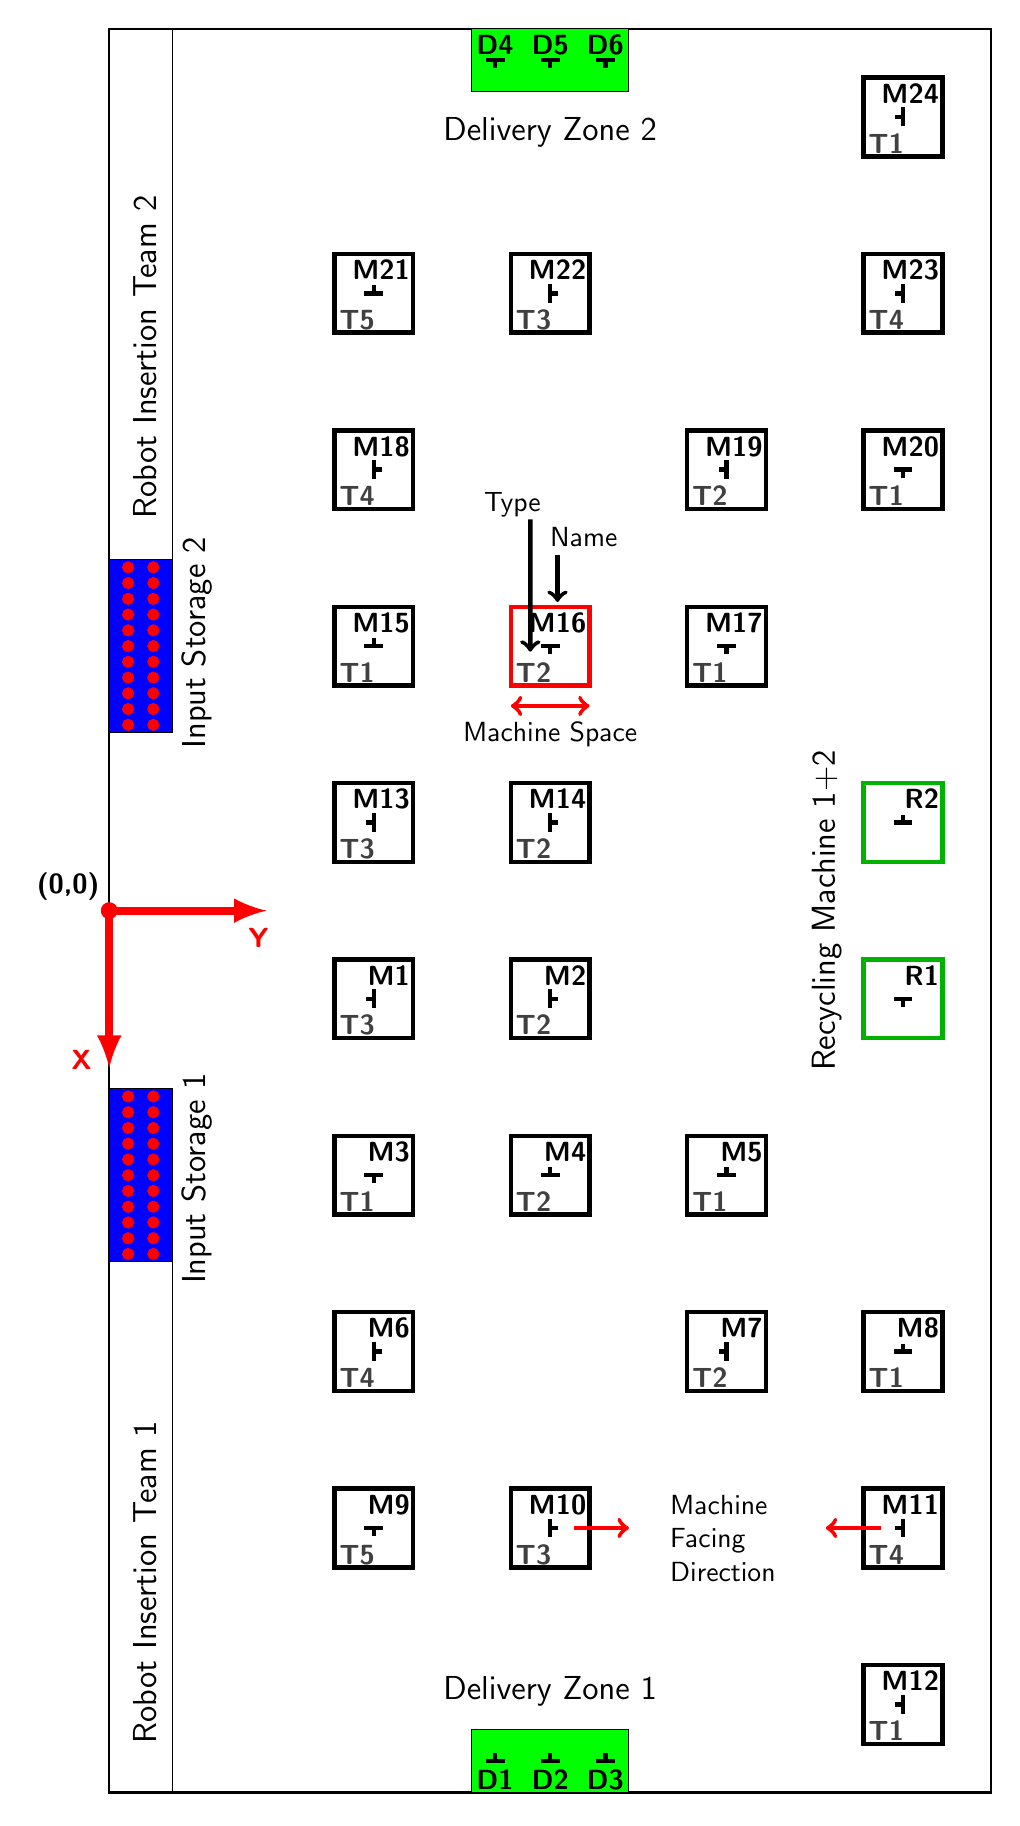
\begin{tikzpicture}[scale=2.0]

	% ATTENTION: the coordinate system here is as follows: nullpoint in the left-bottom-corner; x pointing to the right, y upwards
  
    % field outline
    \draw [thick] (0,0) rectangle (5.6,11.2);
    %\draw [fill=black!8] (0,0.4) rectangle (5.6,5.2);
    %\draw [fill=black!8] (0,0) rectangle +(0.4,11.2);
    %\draw [fill=black!8] (5.2,0) rectangle +(0.4,5.6);

    % coordinate system and origin
    \draw [line width=3pt,red,>=latex,->] (0,5.6) -- +(1,0);
    \draw [line width=3pt,red,>=latex,->] (0,5.6) -- +(0,-1);
    \node [red,anchor=north] at (0.95, 5.55) {\sffamily\textbf{Y}};
    \node [red,anchor=east] at (-0.05, 4.65) {\sffamily\textbf{X}};
    \node [anchor=north east] at (0,5.9) {\sffamily\textbf{(0,0)}};
    \draw (0,5.6) [fill=red,draw=red] circle (0.05);

    % margin areas
    %\draw (5.2,0) -- (5.2,5.6);
    \draw (0.4,0) -- (0.4,3.92);
    \draw (0.4,7.28) -- (0.4,11.2);
    \draw (2.3,0) [fill=green] rectangle +(1,0.4);
	\draw (2.3,10.8) [fill=green] rectangle +(1,0.4);
    \draw (0,3.37) [fill=blue] rectangle +(0.4,1.1);		% was 2.3
    \draw (0,6.73) [fill=blue] rectangle +(0.4,1.1);

    \foreach \m/\t/\x/\y/\ori/\paintbox in
    % row 1
    { M1/3/1.68/5.04/180/1, M2/2/2.80/5.04/0/1, R1/3/5.04/5.04/-90/4,
    % row 2
      M3/1/1.68/3.92/-90/1, M4/2/2.80/3.92/90/1, M5/1/3.92/3.92/90/1,
    % row 3
      M6/4/1.68/2.80/0/1, M7/2/3.92/2.80/180/1, M8/1/5.04/2.80/90/1, 
    % row 4
      M9/5/1.68/1.68/-90/1, M10/3/2.80/1.68/0/1, M11/4/5.04/1.68/180/1, 
    % row 5
      M12/1/5.04/0.56/180/1,
    % Team 2:
    % row 5
      M13/3/1.68/6.16/180/1, M14/2/2.80/6.16/0/1, R2/3/5.04/6.16/90/4, 
    % row 6
      M15/1/1.68/7.28/90/1, M16/2/2.80/7.28/-90/1, M17/1/3.92/7.28/-90/1,
    % row 7
      M18/4/1.68/8.40/0/1, M19/2/3.92/8.40/180/1, M20/1/5.04/8.40/-90/1, 
    % row 8
      M21/5/1.68/9.52/90/1, M22/3/2.80/9.52/0/1, M23/4/5.04/9.52/180/1, 
    % row 9
      M24/1/5.04/10.64/180/1,
    % delivery stations
      D1/D/2.45/0.2/90/2, D2/D/2.80/0.2/90/2, D3/D/3.15/0.2/90/2,		%0.26 instead of 0.2?!
      D4/D/2.45/11.0/-90/3, D5/D/2.80/11.0/-90/3, D6/D/3.15/11.0/-90/3%	%(respectively)
    }
    {
      \draw [ultra thick] (\x,\y) -- +($ (\ori-90:0.06)$);
      \draw [ultra thick] (\x,\y) -- +($ (\ori+90:0.06)$);
      \draw [ultra thick] (\x,\y) -- +(\ori:0.05);
      \if\paintbox1
        \draw [ultra thick] ($ (\x,\y) - (0.25,0.25) $) rectangle +(0.5,0.5);
        \draw [anchor=north east,inner sep=1pt] ($ (\x,\y) + (0.25,0.23) $)
          node (\m) {\fontsize{10pt}{10pt}\selectfont\sffamily\textbf{\m}};
        \draw [anchor=south west,inner sep=1pt] ($ (\x,\y) + (-0.24,-0.25) $)
          node (\m-\t) {\fontsize{10pt}{10pt}\color{black!75}\selectfont\sffamily\textbf{T\t}};
      \fi
      \if\paintbox2
          \draw [anchor=north,inner sep=3pt] ($ (\x,\y) + (0,0) $)
            node (\m)
            {\fontsize{10pt}{10pt}\selectfont\sffamily\textbf{\m}};
      \fi
      \if\paintbox3
          \draw [anchor=south,inner sep=2pt] ($ (\x,\y) + (0,0) $)
            node (\m)
            {\fontsize{10pt}{10pt}\selectfont\sffamily\textbf{\m}};
      \fi
      \if\paintbox4
        \draw [ultra thick] ($ (\x,\y) - (0.25,0.25) $) [draw=black!30!green] rectangle +(0.5,0.5);
        \draw [anchor=north east,inner sep=1pt] ($ (\x,\y) + (0.25,0.23) $)
          node (\m) {\fontsize{10pt}{10pt}\selectfont\sffamily\textbf{\m}};
      \fi
    }

    % Pucks at Zone 1
    \foreach \x in {1,2,...,11}
    {
      \draw ($ (0.12,3.32) + (0,\x*0.10) $) [fill=red,draw=red] circle (0.035);
      \draw ($ (0.28,3.32) + (0,\x*0.10) $) [fill=red,draw=red] circle (0.035);
    }
    
    % Pucks at Zone 2
    \foreach \x in {1,2,...,11}
    {
      \draw ($ (0.12,6.68) + (0,\x*0.10) $) [fill=red,draw=red] circle (0.035);
      \draw ($ (0.28,6.68) + (0,\x*0.10) $) [fill=red,draw=red] circle (0.035);
    }
    
    %\draw (2.24,3.36) [fill=none,draw=red] circle (0.225);	% new Robotino 3.0
    %\draw (3.36,2.8) [fill=none,draw=red] circle (0.185);	% old Robotino 2.0

    \node [anchor=south west,rotate=90] at (0.36,0.25) {\large\sffamily Robot Insertion Team 1};
    \node [anchor=south west,rotate=90] at (0.36,8.03) {\large\sffamily Robot Insertion Team 2};
    \node [anchor=north,rotate=90] at (0.4,3.9) {\large\sffamily Input Storage 1};
		\node [anchor=north,rotate=90] at (0.4,7.3) {\large\sffamily Input Storage 2};
		
    \draw [<->,red,thick,ultra thick] (2.55,6.90) -- +(0.5,0);
    \draw [ultra thick,red] ($ (2.80,7.28) - (0.25,0.25) $) rectangle +(0.5,0.5);
    \node [anchor=north] at (2.80,6.86) {\sffamily Machine Space};

    \node [anchor=north] at (2.8,0.8) {\large\sffamily Delivery Zone 1};
		\node [anchor=north] at (2.8,10.7) {\large\sffamily Delivery Zone 2};
		
		\node [anchor=north,rotate=90] at (4.4,5.6) {\large\sffamily Recycling Machine 1+2};

    \draw [->,red,ultra thick] (2.95,1.68) -- +(0.35,0);
		\draw [->,red,ultra thick] (4.90,1.68) -- +(-0.35,0);
    \node [anchor=south west,text width=1cm] at (3.5,1.28) {\sffamily Machine\\Facing\\Direction};

    % Name/Type explanation and arrows
    \node (name) [anchor=base west,inner sep=0pt] at ($ (M16.north) + (-0.05,0.4) $) {\sffamily Name};
    \node (type) [anchor=base east,inner sep=0pt] at ($ (M16-2.north) + (0.05,0.94) $) {\sffamily Type};
    \draw [->,black,ultra thick] ($ (name.base west) + (0.05,-0.05) $) -- ($ (M16.north) + (0,0.05) $);
    \draw [->,black,ultra thick] ($ (type.base east) + (-0.07,-0.05) $) -- ($ (M16-2.north) + (-0.02,0.05) $);

  \end{tikzpicture}
  \caption{Competition Area}
  \label{fig:competition-area}
\end{figure}

The center coordinates and alignment of the machine and the different
delivery gate slots are presented in Table~\ref{tab:coordinates}. Note
that this field layout should be seen as a proposal for the actual
competition area layout, accounting for symmetry and avoiding
clustering of machine access nodes and unapproachable
machines. However, in case of comprehensible reasons (e.g. hardware or
exhibition issues), the field layout can still change before the
actual tournament starts. Thus, teams should focus on a generic
approach for production, allowing for easy adaptation of machine
positions and alignments.

\begin{figure}
\begin{floatrow}
\begin{minipage}[b]{0.9\linewidth}
  \capbtabbox{%
    \centering
    \mytable{
    \begin{tabularx}{\linewidth}{ll|R|R|R}
      Abbr. & \multicolumn{1}{l}{Type} & \multicolumn{1}{r}{$x$~[\si{\metre}]} & \multicolumn{1}{r}{$y$~[\si{\metre}]} & \multicolumn{1}{r}{Alignment}\\ \hline
      M1 / M13 & Prod. Machine & $\pm$ 0.56 & 1.68 & West \\
      M2 / M14 & Prod. Machine & $\pm$ 0.56 & 2.80 & East \\
      M3 / M15 & Prod. Machine & $\pm$ 1.68 & 1.68 & South / North \\
      M4 / M16 & Prod. Machine & $\pm$ 1.68 & 2.80 & North / South \\
      M5 / M17 & Prod. Machine & $\pm$ 1.68 & 3.92 & North / South \\
      M6 / M18 & Prod. Machine & $\pm$ 2.80 & 1.68 & East \\
      M7 / M19 & Prod. Machine & $\pm$ 2.80 & 3.92 & West \\
      M8 / M20 & Prod. Machine & $\pm$ 2.80 & 5.04 & North / South \\
      M9 / M21 & Prod. Machine & $\pm$ 3.92 & 1.68 & South / North \\
      M10 / M22 & Prod. Machine & $\pm$ 3.92 & 2.80 & East \\
			M11 / M23 & Prod. Machine & $\pm$ 3.92 & 5.04 & West \\
			M12 / M24 & Prod. Machine & $\pm$ 5.04 & 5.04 & West \\
      R1 / R2 & Recycling Machine & $\pm$ 0.56 & 5.04 & South / North \\
      D1 / D4 & Delivery Gate Slot & $\pm$ 5.34 & 2.45 & North / South \\
      D2 / D5 & Delivery Gate Slot & $\pm$ 5.34 & 2.80 & North / South \\ 
      D3 / D6 & Delivery Gate Slot & $\pm$ 5.34 & 3.15 & North / South \\
    \end{tabularx}  
}
  }{%
    \caption{Coordinates and alignment of machines and delivery gate slots}
    \label{tab:coordinates} %
  }

  \end{minipage}
\end{floatrow}
\end{figure}


\begin{figure}
  \subfigure[Puck]{
    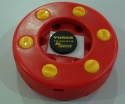
\includegraphics[width=0.2\textwidth]{125px-Puck}
    \label{fig:puck}
  }
  \quad\quad
  \subfigure[Machine]{
    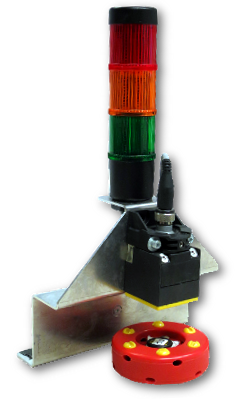
\includegraphics[width=0.2\textwidth]{llsf-signal}
    \label{fig:machine}
  }
  \caption{Hardware equipment used within the competition field.}
  \label{fig:puck-machine}
\end{figure}


\subsection{The Pallet Carrier Puck}
The data-carrying RFID tag is attached on top of a hockey puck. Each
pallet carrier can be identified by a unique number. The tournament puck
features a diameter of \SI{7.5}{\centi\metre} and is shown in
Figure~\ref{fig:puck}. Please consult Appendix~\ref{sec:data-carrier} for
further information of the RFID tag.


\subsection{Machines}
\label{sec:machines}

\subsubsection{General Information}
All machines are identical devices consisting a plate housing the RFID
read/write device and a signal unit according to
Figure~\ref{fig:machine}. They share the same design and RFID
device. The overall size is \SI{280 x 160 x 100}{\milli\metre} (height
$\times$ width $\times$ depth). Confer also
Appendix~\ref{sec:engref} for further details. Machines can be in
different states, which are communicated by their signal lights.

The machine distribution (number of machines per type and team), their
input(s) and output and their range of processing times is summarized
in Table~\ref{tab:production-machines-function}. The machines are
evenly divided among both playing teams. Delivery and recycling
machines for a team are always on the same side as its robot insertion
area and raw input storage.

\subsubsection{Machine Swapping}
\label{sec:machine-swapping}
Depending on the tournament phase
(cf. \refsec{sec:tournament-phases}), some machines are swapped. That
is, some machines are exchanged among the teams, so that a team's
machine is on the half distant from its own delivery gates. For
example, if in \reffig{fig:competition-area} machine M9 would be
chosen, then team 1 would need to use M21, and team 2 would need to
use M9 respectively (the type remains unchanged).

\paragraph{Round-robin phase.~}
One machine type out of the set ${T_3, T_4, T_5}$ is chosen
randomly. All machines of that particular type are swapped.

\paragraph{Play-offs.~}
Half of all machines (of any type) will be chosen randomly and
swapped.

\paragraph{Finals.~}
For each machine (of any type) the referee box will randomly determine
if it is swapped.

\begin{table}[tp]
\centering
	\mytable{  \begin{tabularx}{\linewidth}{l|X|X|X|l}
    \multicolumn{1}{l}{ Type} & \multicolumn{1}{l}{Distribution / Team} & \multicolumn{1}{l}{Input} & \multicolumn{1}{l}{Output} & \multicolumn{1}{l}{(Final) processing time[s]}\\\hline
    \T1 & 4 times & \s0 (raw-material) & \s1 & $t_1 = 3 \mbox{ to } 8~\mathrm{sec}$\\
    \T2 & 3 times & \s0; \s1 & \s2; one consumed container & $t_2 = 15 \mbox{ to } 25~\mathrm{sec}$\\
    \T3 & 2 times &	\s0; \s1; \s2 & \p1; two consumed containers &$t_3 = 40 \mbox{ to } 60~\mathrm{sec}$\\
    \T4 & 2 times & \s0; \s1; \s2 & \p2; two consumed containers &$t_4 = 40\mbox{ to } 60~\mathrm{sec}$\\
    \T5 & 1 times &	\s0 & \p3 &$t_5 =20\mbox{ to } 40~\mathrm{sec}$
  \end{tabularx}}
  \caption{Production Machines - Type, Distribution and working method}
  \label{tab:production-machines-function}  
\end{table}

\subsubsection{Production Machines - During Exploration Phase}
\label{sec:production-machines-exp}
During the exploration phase the robots of each team have to explore
their unknown factory environment, i.e. identify the types of the
different production machines within the competition area. The
frequency of machine types for each team is defined in
Table~\ref{tab:production-machines-function}. The machines will
indicate their different types by individual light signals. In total
there are seven light signals possible with at least one LED switched
on (no flashing lights). The light signals and the corresponding
machine types are initially unknown. The Referee Box will assign every
machine type to a light signal and publish it to the robots. The
exploration phase starts with the announcement of the exploration game
phase by the Referee Box. An exploration information message is sent,
which defines the light signals of the machine types, e.g., red and
green LED switched on indicate machine type \T1. If a robot perceives
the red and green LED light switched on at machine \m1, the robot has
to announce that machine \m1 is of type \T1 to the Referee
Box. Therefore, the robot has to send a \emph{machine identified
  message} to the Referee Box. Please consult the RoboCup Logistics
League Referee Box Integrator's Manual for a detailed definition of
the message types.

\begin{table}[tp]
\centering
\mytable{\begin{tabularx}{\linewidth}{p{0.35\linewidth}|X}
		\multicolumn{1}{l}{Optical Feedback} & \multicolumn{1}{l}{Operating mode} \\ \hline 
				All LEDs turned off &  	The machine is physically offline, caused by a real error, which should not happen during the competition. \\
					Red LED turned on &  	The machine is out of order. \\
					Green LED turned on &  	The machine is idle and ready.\\
					Green and yellow LED turned on &  	The machine is processing or consuming the current data carrier. \\
					Yellow LED flashing (at 2 Hz) & The machine detects wrong material.
					This can be caused by data carriers that are already consumed,
					sub-assemblies that do not fit to this machine type's work order or
					corrupted data carriers. \\
					Red and yellow LED flashing (at 2 Hz) & The machine detects a data carrier, which belong to the opposing team. \\%\hline
	\end{tabularx}}
  \caption{Production Machines - Optical Feedback during production phase}
  \label{tab:production-machines-feedback}  
\end{table}


\subsubsection{Production Machines - During Production Phase}
The default operating mode of all machines implies that only the green
LED is turned on. This signals that the machine is ready for input.
To enable the production process it is necessary to transport the
pallet carrier accurately to the RFID device.
% we will not write anymore to the puck, we're safe
% The reading and writing process is a delicate process.  To avoid
% corruption of the data carrier, it should not leave the working
% range of the RFID device once the processing or consuming is
% started.

If a (intermediate) product is fed into a machine, the machine reads
the RFID tag and checks whether or not the product can be processed
and indicates the result by its signal light. If an appropriate
product is fed to the machine, the yellow LED turns on indicating that
the machine is processing the product (green and yellow LED on). If
the machine needs another sub-assembly to generate an output, the
green LED turns off and the yellow light indicates that the machine is
waiting for the next sub-assembly. A consumed pallet carrier has to
stay within the machine space borders (no part of the puck being
outside the mark-up, note that if the overhead camera system is used
there might be a small tolerance, but the team may not rely on this)
until the production cycle of that very machine has been completed.
Products resulting from violating this requirement are considered junk
and will not be rewarded.

If the yellow LED is turned off after processing, further input
materials are fed to the machine, the green LED indicates that the
machine has finished the work order and the last carrier is
transformed to its corresponding output.

If a product is fed to a machine which is not appropriate, the machine
reacts with a yellow light flashing at 2 Hz. A red light indicates
that the machine is in an error state.  In this case no products can
be processed on the machine (for details
cf.~\refsec{sec:out-of-order}). In case a data carrier is fed to a
machine, which belongs to the opposing team, the red and the yellow
LEDs are flashing at 2 Hz and the puck is marked as junk.
Table~\ref{tab:production-machines-feedback} summarizes the operating
modes of the production machines and the corresponding signal lights.

The machine always processes the required pallet carrier delivered
last, all prior components will be consumed. All machines will start
processing the data carrier as soon as it enters the machine zone as
stated in Section~\ref{sec:competition-area}. They will change their
operating mode according to
Tables~\ref{tab:production-machines-feedback},
\ref{tab:recycling-machine}, and \ref{tab:delivery-gates}.

In order to complete the machines' work order, the input materials have
to be delivered one-by-one into the RFID device's action range. The
sequence of delivered input materials is irrelevant (e.g., \s0-\s1 or
\s1-\s0). Multiple data carriers in range of the device will result in
erroneous behavior of the device. Consumption of materials, such as
\s0 used in the production of \s2, will take 2 seconds. Unloading the
machine can be done immediately after the operating mode changes away
from processing. As long as the machines are used properly, they will
not produce any junk. The distribution describes how many machines of
the respective types will be randomly placed resulting in a total of
12 court machines for each team.

\subsubsection{Recycling Machines}
During the staged production process raw-material is transformed or
consumed by the machines. To use consumed raw-materials again, the
robots of each team can use their corresponding recycling machine
(i.e., R1 for team 1 and R2 for team 2).  The recycling machine
processes all supplied loading carriers back to raw-material (\s0)
within 2 seconds. The optical feedback provided by the recycling unit
differs from production machines and is shown in
Table~\ref{tab:recycling-machine}.

\begin{table}[tp]
  \centering
  \mytable{\begin{tabularx}{\linewidth}{p{0.35\linewidth}|X}
      \multicolumn{1}{l}{Optical Feedback} &\multicolumn{1}{l}{Operating
        mode}\\\hline
      All LEDs turned off & 	The machine is physically offline,
      caused by a real error, which should not happen during the
      competition.\\
      Red LED turned on & 	The machine is out of order\\
      Green LED turned on & 	The machine is idle and ready.\\
      Green and yellow LED turned on & The machine is processing the
      current data carrier.\\
      Red and yellow LED flashing (at 2 Hz) & The machine detects a
      data carrier which belongs to the opposing team. \\%\hline
  \end{tabularx}}
  \caption{Recycling Machines - Optical Feedback}
  \label{tab:recycling-machine}
\end{table}

\subsubsection{Delivery Gates} 
\label{sec:delivery-gates}
If a team finishes a variant of a final product, it has to be
delivered to the customer through one of their three delivery
gates. Only if the machine signals successful delivery (all lights
steadily on) points are awarded. This state will last until the puck
is removed by the referee. The puck may no longer be used in the
game. There will be only one active gate at a time for each team. A
gate is active between 60 and 180 seconds. After the gate switches,
there is a grace period of 3 seconds, in which delivery will still be
accepted to the formerly active delivery gate. False deliveries to an
active gate will be indicated by a flashing yellow light (e.g. taking
a \s0 puck to the active gate) and false deliveries to an inactive
gate by a steady red and blinking yellow light. In both cases, the
puck will be taken out by the referee and it may no longer be used in
production or delivered. In case of a delivery to an active gate, the
team will be awarded with the points for the delivery; if the gate was
inactive, no points will be awarded. If, however, a pallet carrier was
not successfully delivered, the pallet carrier will remain where it
is. See Table~\ref{tab:delivery-gates} for the possible delivery gate
signal states.

\begin{table}[tp]
  \centering
  \mytable{\begin{tabularx}{\linewidth}{p{0.35\linewidth}|X}
      \multicolumn{1}{l}{Optical Feedback} &\multicolumn{1}{l}{Indication}\\\hline
      Red turned on & This delivery gate is inactive.\\
      Green turned on & This gate is active, namely the
      designated gate.\\
      Yellow blinking & False delivery to active gate.\\
      Red on, yellow flashing (at \SI{2}{\hertz}) &
      False delivery to inactive gate.\\
			Red and yellow LED flashing (at 2 Hz) & False delivery with a data carrier belonging to the opposing team. \\
      Red, yellow, and green turned on & Successful delivery.\\
%    \hline
  \end{tabularx}}
  \caption{Delivery Gates - Optical Feedback}
  \label{tab:delivery-gates}
\end{table}

%%%%%%%%%%%%%%%%%%%%%%%%%%%%%%%%%%%%%%%%%%%%%%%%%%%%%%%%%%%%%%%%%%%%%%%%%%%%%
%%%

\section{Referees}
Referees manage the overall game, make sure that the rules of the game
are followed, and instruct and monitor the referee box. In this
section, we will describe their duties and responsibilities in more
detail.

\subsection{Referee Delegation}
Each participating team of the tournament must provide at least two
team members which act as referees. These referees must be announced
at the beginning to the tournament and are fixed throughout the whole
competition (unless the participant drops out of the tournament,
e.g. because of illness). The referees must meet the following
criteria. They must

\begin{itemize}
  \item be available for each game that they are assigned to
    and appear 5 minutes prior to the game start time (schedule will
    be announced by Organizing Committee at beginning of tournament)
  \item have good knowledge of the rulebook and the applied rules
  \item participate in the referee briefing at the beginning of the
    tournament (organized by the Organization and Technical
    Committees)
  \item be able to lead a game and communicate with the teams in
    English.
\end{itemize}

\subsection{Tasks and Responsibilities}
Each game requires 3 referees. One referee will run and oversee the
referee box. Two field referees observe the field, announce rule
violations, and communicate with the teams and refbox referee. Each
field referee is assigned to a particular field half. The referee
named first on the schedule is the head referee. The head referee has
the upper hand when there is a referee disagreement and then announces
the final decision.

The refbox referee has to operate the control machine during the game,
observe its status to ensure the correctness of the digital
representation and automatic scoring, announce critical situations to
the field referees, and start and stop the game on request of the
field referees. The refbox referee must also enter robot restarts and
observe the time remaining to bring back a robot, or announce if a
robot may no longer participate in the game (second restart).

The field referees observe the game from the side of the field or from
any position on the field (e.g. to better understand the game
situation). They shall avoid robots spatially on the field, but
ultimately robots are expected to avoid collision with human
referees. Field referees are also responsible for re-positioning pucks
after pushing or remove pucks that were delivered to a delivery gate
if and only if the delivery gate as either accepted (all LED steady
on) or rejected (yellow blinking with or without red light on). Field
referees are responsible for making the decision whether a team may
take out a robot for maintenance.

Each referee may call a pause of the game at any time, e.g. if robots
must be penalized or disentangled after a collision. Referees may
explicitly pause the game to convene and discuss an unclear situation
as to avoid hasty decisions. Such pauses shall be short-lived as to
follow the competition schedule. %  there is an unclear situation, or

\subsection{Liability Waiver}
Referees cannot be held liable for:
\begin{itemize}
\item any kind of injury suffered by a player, official or spectator
\item any damage to property of any kind
\item any other loss suffered by any individual, club, company,
  association or other body, which is due or which may be due to any
  decision, which he may take under the terms of the Laws of the Game
  or in respect of the normal procedures required to hold, play and
  control a match.
\end{itemize}

\subsection{Complaint Procedure}
Rule issues are not to be discussed during a game. Referee decisions
are binding for the game. A team may protest and challenge a game by
executing the following complaint procedure. The procedure is also
automatically invoked if a referee decides to abort a game for any
reason (e.g. field damage, lighting failures, burning robots).

To initiate the complaint procedure, the team leader of the
challenging team is to contact a member of the Technical Committee
within 10 minutes after the respective game has ended. The member of
the Technical Committee then invokes a team leader conference in
cooperation with the Organizing Committee. In this conference, the
following parties participate: the referees of the game in question,
not less than half of all registered team leaders, and the Technical
Committee (counseling). The situation shall be resolved by unanimous
consent or by vote of the team leaders (majority of team leaders
participating in the conference is sufficient).

All teams are reminded that while this is a competition, the league is
also about \emph{cooperative} research and evaluation and complaints
should be handled in a fair and forthcoming way.

\section{Game Play}
A match is defined by two contesting teams competing within the same
identical competition area. Each team consists of a maximum of 3
robots. Each match consists of 5 minutes of setup time, a maximum of 4
minute exploration phase, and a 15 minute production phase.
The three phases of the game are detailed below.

\subsection{Environment Setup}
\label{sec:env-setup}

The physical distribution and alignment of the production machines is fixed. The machine
type of each production machine will be randomized prior to each
match. The processing time of each machine type will be determined in
the same way, so the waiting time during a match will be static for
each machine of all machine types (e.g. all T1 could have 7 seconds
processing time). The active delivery gate will also be randomized
prior to each match, but during a match the active gate can switch. At
the beginning, 22 raw materials (pucks in $S_0$ state) will be placed
in each input storage, initially spread as shown in
\reffig{fig:competition-area}. The pucks may only be touched by a
robot after the game has started. In particular, they may not be
re-positioned for better alignment if they have been pushed or moved by
a robot during the game.

\subsection{Game Phases}
\label{sec:game-phases}

\subsubsection{Team Setup}
\label{sec:team-setup}
No team member is allowed to enter the competition area prior to or
during a match. All robots which are to participate in the game, need
to be in the game area during setup. All robots are allowed to roam
through the entire area, autonomously or teleoperated. However, no
robot is allowed to touch any pallet carrier during setup;
infringements will be punished as \textit{misbehaving robot}. The
referee box will control the setup period. When the game starts, all
robots need to be in the insertion area; no robot is allowed to be in
the factory area at start-up. If a robot is not able to move to the
insertion area, the team has to call upon the referee for
\textit{robot maintenance}.


% The robots can be set up within the factory area and have not been
% elevated into their autonomous state. Any necessary setup routine can
% be performed. This includes, but is not limited to, remote start-up of
% programs, localization procedures, or vision calibration.

\subsubsection{Interruptions and Robot Maintenance}
\label{sec:robot-maintenance}
During a match and while the robot is active on the field no manual
interference or manipulation of the robot in hardware, software,
configuration, instructions, or whatsoever, is allowed.

% In the case of a misbehaving or broken robot, a team can ask the
% referee to take out a robot. Note, however, that one robot interfering
% with another is no conduct of misbehavior (unless damage is to be
% expected) and no reason to call out a robot. Similarly, to ask to take
% out a robot which is in a software deadlock situation of the own
% control software is not judged as a broken robot. The final decision
% whether a robot can be taken out or not remains with the field
% referee. The referee acts upon this motion at a time of his choosing,
% but as soon as possible.

Each team is allowed to maintain each robot once per game. The team
has to call upon the referee for \textit{robot maintenance}. The
referee should judge the game situation carefully and should allow the
robot to be taken out for maintenance, if neither the calling team
nor another robot would have any advantage in the current game
situation from the take-out. An advantage would be, for instance, to
take out a robot, if two robots are hindering each other. It is up to
the discretion of the referee when to allow the robot maintenance.


After a robot has been taken out for the first time, it is handed to
the team. The team can perform any repairs to the robot and/or the
robot's software. %on the robot which is limited
%to adjustments on sensors, checking cable connections, or restarting
%the robot's control software. 
The repair time may take at most 120 seconds. If the robot is not
returned to the field in time, it is disqualified from the ongoing
game.

To return the robot into the game, the team asks the referee to place
back the robot onto the field. After the referee accepts the motion,
the robot is placed in the robot insertion area. The team has 15
seconds quick setup time, which is limited to basic instructions like
initial localization or software start-up.

The referee can interrupt the game at any point in time, but should do
so rarely as not to interfere with the overall game flow (also
cf.~\refsec{sec:during-match}).
% The referee can also decide to take
%out a robot if it is not moving at all for more than 120 seconds and
%seemingly not waiting at a game relevant place, e.g. at a temporarily
%out-of-order machine, or if it may harm or damage the field or other
%robots.

If a robot needs to be taken out for the second time, either on
request or as decided by the referee, it is disqualified from the
current game. It may no longer communicate with the still active
robots and must be taken out of the competition area.

\subsubsection{Game Start}
\label{sec:game-start}
%
All matches will start at the exact time scheduled by the organization
team. From this point on, all robots must be located within the robot
insertion area and the teams involved are allowed to start their
robots to work autonomously within one minute (the game time will
already start during this time). This can be done by issuing one
single distinct command via any kind of interface or pressing a single
button on the robot.

\subsubsection{Exploration Phase}
\label{sec:expphase}
%
With the start of the game, the exploration phase begins. All machines
indicate their type using steady light signals. The signal light
encoding of machine types will be published by the referee box as
described in \refsec{sec:production-machines-exp} and in detail in the
RoboCup Logistics League Referee Box Integrator's Manual. The robots
are to roam the environment and announce the detected types of their
12 production machines to the referee box.  Each properly reported
signal scores \num{+4} points, each signal reported wrongly will give
\num{-3} points penalty. A minimum of zero points will be accounted
for this exploration phase. Production or moving pucks is not allowed
during the exploration phase.  The exploration phase ends either after
four minutes or immediately after all 12 machines have been reported
by both teams.



\subsubsection{Production Phase}
\label{sec:production-phase}

With the end of the exploration phase, the actual production begins,
which lasts \num{15} minutes. The referee box publishes all information
regarding products and machines. This includes position, orientation,
and type of each machine, as well as the different product variants
that can be produced.


\subsection{Production Portfolio}
\label{sec:prodportfolio}

The production portfolio is presented in
Figure~\ref{fig:production-diagram}, which shows a production chain
diagram with the machines and their respective inputs and outputs. The
multistaged production processes can be repeated as long as enough
pallet carriers can be provided to complete the cycle. The different
machine types are specified in Section~\ref{sec:machines}.


% \begin{figure}[tbhp]
%   \centering

% \tikzstyle{M}=[rectangle, draw=blue, thick, fill=blue!20, text width=2em,align=center, rounded corners, 
%   minimum height=2em]
% %
% \tikzstyle{P}=[draw=red, thick, circle,fill=red!20, minimum height=1.5em]

% \begin{tikzpicture}[level distance=4em,sibling distance=5em]
%   \node[P] {$S_1$}  [grow=left,thick]
%   child { node[M] {$M_1$}
%     child { node[P] {$S_0$}}};
% \end{tikzpicture}
% \hspace*{1em}
% \begin{tikzpicture}[level distance=4em,sibling distance=5em]
%   \node[P] {$C$}  [grow=left,thick]
%   child { node[M] {$M_1$}
%     child { node[P] {$S_0$}}};
% \end{tikzpicture}

% \begin{tikzpicture}[level distance=4em,sibling distance=5em]
%   \node[P] {$C$}  [grow=left,thick]
%   child { node[M] {$M_2$}
%     child { node[P] {$S_0$}}
%     child { node[P] {$S_1$}}
%     child { node[P] {$S_2$}}
%     };
% \end{tikzpicture}

% \begin{tikzpicture}[node distance=4em,level distance=4em,sibling distance=5em]

%   \node[P] (p) {$P$}  [grow=left,thick]
%   child { node[M] (m) {$M_3$}
%     child { node[P] {$S_0$}}
%     child { node[P] {$S_1$}}
%     child { node[P] {$S_2$}}
%    };
  
% \end{tikzpicture}


%   \caption{The production diagram}
% \label{fig:production-diagram}  
% \end{figure}





%\begin{figure}
%\begin{floatrow}
%  \capbtabbox{%
%    \centering
%    \mytable{\begin{tabularx}{\textwidth}{C|C|C|c}
%        \multicolumn{1}{c}{Sub-assembly} & \multicolumn{1}{c}{Deployable} & \multicolumn{1}{c}{Prerequisites} & \multicolumn{1}{c}{Result}\\\hline
%        \s{0} &	\T{1}, \T{2}, \T{3}, \T{4}, \T{5} & none & \s{1}, \p{3} or
%        \TAG{consumed}\\
%        \s{1} &	\T{2}, \T{3}, \T{4} &  	\s{0} & 	\s{2} or \TAG{consumed} \\
%        \s{2} & \T{3}, \T{4} & \s{0}, \s{1} &	\p{1}, \p{2} \\
%%        \hline
%      \end{tabularx}
%    }      
%  }{%
%    \caption{Production table}
%    \label{tab:production-table}
%  }
%\end{floatrow}
%\end{figure}
  
\begin{figure}
  \ffigbox{%
    \centering
    
    \tikzstyle{M}=[rectangle, draw=blue!50, thick, fill=blue!20, text width=2em,align=center, rounded corners=2pt, 
    minimum height=2em]
    % 
    \tikzstyle{P}=[draw=orange, thick, circle,fill=orange!20, minimum height=1.5em]
    
    \hfill
    \begin{minipage}[b]{0.26\linewidth}
      \subfigure[$P_3$]{\label{fig:prod-chain-S1a}%
        \begin{tikzpicture}[level distance=4em,sibling distance=5em,draw=orange!80]
          \node[P] {$P_3$}  [grow=left,thick]
          child { node[M] {$T_5$}
            child { node[P] {$S_0$}}};
        \end{tikzpicture}
      }

      \medskip

      \subfigure[$S_1$]{\label{fig:prod-chain-S1b}%
        \begin{tikzpicture}[level distance=4em,sibling distance=5em,draw=orange!80]
          \node[P] {$S_1$}  [grow=left,thick]
          child { node[M] {$T_1$}
            child { node[P] {$S_0$}}};
        \end{tikzpicture}%
      }
    \end{minipage}
    \hfill
    \subfigure[$S_2$]{\label{fig:prod-chain-S2}%
      \begin{tikzpicture}[level distance=4em,sibling distance=4em,draw=orange!80]
        \node[P] {$S_2$}  [grow=left,thick]
        child { node[M] {$T_2$}
          child { node[P] {$S_0$}}
          child { node[P] {$S_1$}}
        };
      \end{tikzpicture}
    }
    \hfill\,

    \bigskip

    \hfill
    \subfigure[$P_1$]{\label{fig:prod-chain-P1}%
      \begin{tikzpicture}[node distance=4em,level distance=4em,sibling distance=4em,draw=orange!80]
        \node[P] (p) {$P_1$}  [grow=left,thick]
        child { node[M] (m) {$T_3$}
          child { node[P] {$S_0$}}
          child { node[P] {$S_1$}}
          child { node[P] {$S_2$}}
        };
      \end{tikzpicture}
    }
    \hfill
    \subfigure[$P_2$]{\label{fig:prod-chain-P2}%
      \begin{tikzpicture}[node distance=4em,level distance=4em,sibling distance=4em,draw=orange!80]
        \node[P] (p) {$P_2$}  [grow=left,thick]
        child { node[M] (m) {$T_4$}
          child { node[P] {$S_0$}}
          child { node[P] {$S_1$}}
          child { node[P] {$S_2$}}
        };  
      \end{tikzpicture}
    }
    \hfill\,
}{%
  \caption{Production Chain Diagrams showing the machines and inputs
    relative to their outputs.}
  \label{fig:production-diagram}  
}
\vspace{-1mm}
\end{figure}
%\todo[inline]{What is a C??}

\subsection{During a Match}
\label{sec:during-match}
Any referee can interrupt the match at any time. After the referee box
is stopped, all robots have 5 seconds to stop all robot movement.
Robots that do not stop within the time limit will be treated in the
same way as misbehaving robots (cf.~\refsec{sec:robot-maintenance}).
The match time will be paused during the interruption.

\subsubsection{Out-of-order}
\label{sec:out-of-order}
The downtime generator will take down machines randomly out of the
pool containing all production machines. It will do so at random
points of time and with the same conditions for both teams, i.e.,
affecting the same machines for both teams. There will be 6 to 8 of
such triggered events during a match. The machines affected will
remain out of order for 30 to 120 seconds. Every machine can only be
forced out of order once per match. The recycling machines will be
taken down exactly once per match, with a downtime of 20 to 40
seconds. If a machine turns offline during processing or consumption
of mounted a pallet carrier, it will afterwards resume the process
(extending the overall processing time by the down time).

\subsubsection{Production Plan}
The referee box will announce orders throughout the game in an
incremental fashion. Each order will consist of the products to
produce, the amount thereof, and delivery time slots. In each game,
orders with a fixed delivery value of 80 points will be
placed\footnote{This number is based on experience from the game
  reports and database logs of the competition in 2013. The number can
  be adjusted during the tournament by the Technical Committee should
  this turns out to be necessary.}. These points only include the the
final production step and delivery. Each order will require one or
more products of a specified product type to be delivered. The
delivery time slot will have a randomized start time and a randomized
duration between 30 to 180 seconds. The end time shall be within the
game time. The duration shall be long enough to cover at least the
production time of the final machine in the production chain and 30
seconds of travel time. The orders shall be posted with a uniform
distribution over the whole game time (but there is not necessarily an
open order for a particular product at a specific time, or any order
at all). The first order will be posted within the first 120 seconds
of the game (but not necessarily at the beginning of the game). An
order will be announced between 10 and 60 seconds before the delivery
time slots starts.

In all tournament phases (cf.~\refsec{sec:tournament-phases}) the
teams playing on the field at the same time will get the same
production plans but other games will have their own.

% \begin{table}[t]
%   \centering
%   \mytable{\begin{tabularx}{\linewidth}{p{0.35\linewidth}|X}
%     \multicolumn{1}{l}{Product variant} &\multicolumn{1}{l}{Demanded number of items } \\
%     \hline 
%     Product variant \p1 &	$N_1 = 1 \mbox{ to } 10$ items \\
%     Product variant \p2 &	$N_2 = 1 \mbox{ to } 10$ items \\
%     Product variant \p3 &	$N_3 = 1 \mbox{ to } 10$ items \\
%     %	\hline
%   \end{tabularx}}
%   \caption{Production plan}
%   \label{tab:production-plan}
% \end{table}

\section{Tournament}
\label{sec:tournament}

\begin{table}
  \centering
  
    \subtable[Scoring scheme for the exploration
  phase]{\mytable{\begin{tabularx}{\linewidth}{p{7em}|X|p{2.4em}}
        \multicolumn{1}{l}{Reported} &\multicolumn{1}{l}{Exploration Phase} & \multicolumn{1}{l}{Points}\\\hline
    Correctly & Correctly determine a machine type and
    report it successfully to the refbox &	+4\\
    Incorrectly & Wrongly reported machine type &  -3\\
    Round Total & A maximum of 48 points can be achieved by correctly
    reporting all 12 production machines. A minimum of 0 points is
    awarded. & 0 -- 48\\%\hline
  \end{tabularx} }}
  
  \bigskip
  
  \subtable[Scoring scheme for the production phase]{\mytable{\begin{tabularx}{\linewidth}{p{7em}|X|p{2.4em}}
        \multicolumn{1}{l}{Sub-task } &\multicolumn{1}{l}{Production Phase} &
        \multicolumn{1}{l}{Points}\\\hline
        Produce \s2 & Finish the work order of a machine type 2 & $+4$\\
        Produce product variant \p1  & Finish the work order of a machine type 3 & $+12$ \\
        Produce product variant \p2  & Finish the work order of a machine type 4 & $+12$ \\
        Produce product variant \p3  & Finish the work order of a machine type 5 & $+0$ \\
        Delivery & Deliver one of the final product variants to the
        designated loading zone at the time specified in the order & $+10$\\
        Wrong delivery & Deliver one of the final product variants to the
        designated loading zone out of the requested time range or after
        all products requested in the period have already been delivered
        & $+1$\\
        False delivery & Deliver an intermediate product & $0$\\
        Just-in-time Production & The final production step of a
        successfully delivered good has been completed within the
        order time window& $+5$\\
        Recycle & Taking a consumed material from a machine that completed
        its work cycle to the recycling machine& $+5$\\
				Obstruction Penalty & Deliver a data carrier to a machine, which belongs to the opposing team. & $-2$ \\
    \end{tabularx}  }}

	\bigskip

	\subtable[Scoring scheme for game commentary]{\mytable{\begin{tabularx}{\linewidth}{p{7em}|X|p{2.4em}} \multicolumn{1}{l}{Task} &\multicolumn{1}{l}{Game Commentary} & \multicolumn{1}{l}{Points}\\\hline
      Accepted Commentary & Commentate at least one half of the game continuously
      on microphone in English to the public. &  +10\\%\hline
  \end{tabularx} }}
  
  \caption{Scoring Schemes}
  \label{tab:scoring}   
\end{table}

\subsection{Tournament Phases}
\label{sec:tournament-phases}
% The tournament features two stages with the first stage being done in
% league form with several sequels orientating at the number of
% participants and a second stage with playoffs featuring the top 4
% teams.

\paragraph{Round-Robin phase} 
There will be three stages in the tournament. The first stage is a
group phase and will be played as a round-robin. The best 4 teams of
the round-robin stage will advance to a playoff round. The best 2
teams of this phase play the final game.

%
At the round-robin stage, the teams will receive the true points they
scored by delivering and producing goods during the competition. The
points will be accumulated in this phase and the teams will be ranked
according to the accumulated points in descending order.

\paragraph{Playoffs}
At the playoff stage, the scoring scheme will be different. As each
team in this phase directly competes with an opposing team, the team
that scores more points as the direct opponent, will be announced as
the winner and 3 points will be awarded to this team. A loss will be
awarded with 0 points. Additionally, if both teams are unable to score
any points during the match by delivering or producing goods, both
teams will receive 0 points.
%
% Each match will be resulted with the score of each team. The winning
% team will be awarded 2 major points. In case of a draw both teams will
% be awarded with 1 major point. In case both teams scored zero points,
% no major points will be awarded.
%
In case of a draw within the playoffs, the game time will be extended
by 5 minutes unless both teams scored zero points. This will be
announced by the refbox instead of a game closed message.
%
If this extension leads to a draw too the overall regular points of
the teams will determine the match winner. If the overall points are
equal too, a direct comparison between the teams in question will
decide. If this fails to resolve the situation, the teams will
approach a coin toss to determine the winner.



\paragraph{Finals.}
The best 2 teams of the playoff phase will advance to the finals.
The two teams compete directly in concurrent games. The team that
scores more points after the regular game time wins. If there is no
winner after the regular time, the game continues for 5 more
minutes. If after this time there is still no winner, a coin toss will
decide.

\bigskip
The detailed seeding will be created at the event. Although the idea
is to allow each participant to challenge each other team the league
can be adjusted to meet time requirements.


\subsection{Game Commentary}
In addition to scoring in the exploration and the production phase,
points are also awarded if a team provides an English commentary on
microphone to the public throughout the game. The commentary should
communicate the overall problems to be solved within this league, the
actual events taking place, but also give an insight on the own team
and how they solved certain tasks. It does neither have to be perfect,
nor to be a flawless stream of information. The commentary should be
continuous, but short pauses are acceptable. At the end of the game
the referees decide if the commentary duties were met and award the
according team with 10 points. If both teams are willing to commentate
on the game, the game time is shared according to the team
specification (e.g., team 1 commentates the first half, team 2 the
second half). The teams can make custom arrangements to split the
overall time.

\subsection{Task Fulfillment and Scoring}
Table \ref{tab:scoring} provides the itemized clearance of all task
related processes and their scoring.

\subsection{Obstruction Penalty}
Teams are penalized with -2 points for obstruction when delivering a
data carrier to a machine of the opposing team.  In this case, the
puck becomes junk and cannot be recycled or used afterwards. If the
robot leaves the machine space without the puck, the puck will be
removed by a field referee.

\subsection{Pushing Rules}
With multiple teams on the field at the same time, robots must
implement ways for collision avoidance. At the same time, they shall
not interfere with the goods of the other team. The case where a robot
of one team bumps into or moves a robot or puck of another team we
call ``pushing''.

The following rules shall be obeyed by the robots and provide the
guidelines for referees to call for improper behavior of a robot due
to pushing.

\begin{enumerate}
\item Pushing occurs only between robots of different teams.
\item Robots must drive such that they try to avoid physical contact
  with robots from the opposing team. However, physical contact per se
  does not represent an offense.
\item All robots should be equipped to detect situations of physical
  contact with other robots (direct pushing situations).
\item If physical contact with other robots cannot be avoided, it must
  be soft, i.e. at slow speed and with as small physical impact as
  possible, in order to avoid damage to itself and other
  robots. Robots moving at high speed must significantly decelerate
  before a collision occurs with another robot.
\item If a destruction collision is immediate and the robots don't
  react, the referee should use the refbox to send a stop command to
  all robots. Every team has to react to the stop command by
  immediately stopping their robots.
\item Whenever a robot produces direct physical contact with another
  robot while moving, it must stop movement immediately in that
  direction (and choose a new direction for movement).
\item If pushing occurs between a moving and a standing robot, the
  moving robot causes the pushing situation and is responsible for
  resolving it. If it is not able to do this, a pushing foul will be
  called.
\item If pushing occurs between two moving robots, both robots are
  responsible for resolving the pushing situation. If one robot
  continues pushing by moving in its initial direction, while the
  other robot is recognizably reacting and trying to take another
  direction, the foul will be called on the pushing robot.
\item If two robots encounter physical contact and cannot resolve the
  situation because they get entangled, the referee may issue a
  pushing foul on both robots.
\item If, in the opinion of the referee, physical contact between two
  robots is not soft, or if one or both of the robots do not change
  direction after encountering physical contact, a pushing foul will
  be called.
\item When a pushing foul is detected the responsible team has to use
  up their restart for the stuck robot to start at the insertion zone
  again. The other team can decide within 10 seconds to restart their
  involved robot in the insertion zone without it counting as a
  penalty restart.
\item Moving a puck of the opposing team within a fenced area (machine
  or input area) by at least one puck diameter is a pushing foul. The
  referee will move the puck back to its original position.
\item If a robot loses his puck during collision avoidance or in case
  of a collision the puck will not be replaced.
\item The league reserves its right to disqualify clearly malicious
  teams.
\end{enumerate}


\subsection{Penalties}
The catalog in Table~\ref{tab:infringements} represents the decision
basis for the referees without being exhaustive or binding.
%

\begin{table}
  \centering
  \mytable{
    \begin{tabularx}{\linewidth}{l|X}
  \multicolumn{1}{l}{Issue} &\multicolumn{1}{l}{Sanction}\\\hline
  Premature movement & No robot is allowed to move until the referee
  announced the start of the match The faulty robot will be grounded
  for 2 minutes.\\[1ex]
%
  Damaging factory equipment & Theoretical damage to the real
  factory equipment as a result of collisions and negligent actions.
  This behavior will be punished as a minor rule break.\\[1ex]
  % The team will be punished with a score reduction. The total score
  % cannot  drop below zero.\\[1ex]
%
  Not showing up & A team not showing up at all. The team will be
  removed from the tournament unless the team leader can provide a
  sincere explanation.\\[1ex]
%
  Manual Interference & A manual interference of a team, i.e. touching
  a robot without the referee's permission, during the game will be
  punished as a major rule break.\\[1ex]
%
  Breaking a minor rule & A rule infringement with minor impact on the
  team performance or competition mechanics. Upon decision of
  the referee, 25 \% of the scored points of the team at the time of
  the infringement will be deducted, at least 1 point.\\[1ex]
  %
  Breaking a major rule & A rule infringement with considerable impact
  on the team performance or competition mechanics. Upon decision of
  the referee, 50 \% of the scored points of the team at the time of
  the infringement will be deducted, at least 5 points. \\[1ex]
  % The referee will
  % decide upon calling a team vote or imposing an adequate punishment.\\[1ex]
  % 
  Arguing with the referee & There will be no discussions during a
  match. Each team can make a motion to protest a certain match and
  its result which will be dealt with after the match. There will be a
  warning. Continued disregard will result in a time punishment to the
  team's current or next match.\\[1ex]
%
  Disregarding rules of conduct & Following the rules of conduct
  should be self-explanatory Upon disregard, the referee will impose
  sanctions ranged from time punishments to the team's complete
  removal from the tournament.\\%\hline
  \end{tabularx}  }
  \caption{Infringements}
  \label{tab:infringements}
    
\end{table}


\subsection{Technical Challenge}
\label{sec:technical-challenge}
Within the league, the technical advances should be documented from
year to year. Therefore, the Technical Challenge is introduced. Each
team should prepare for participating in any number of the following
tasks. However, participation has no influence on the normal game
results, but the winner will be awarded by a certificate.


\subsubsection{Navigation and dynamic collision avoidance}
A robot fleet consisting of three robots has to show that it can reach
a certain goal location avoiding collisions with static obstacles and
other moving robots. Two teams compete against each other at the same
time. Team 1 places their robots inside the competition area with $x >
4.79$m (i.e., near the delivery gate at the bottom), team 2 at $x <
-4.79$m (i.e., near the delivery gate at the top). All robots from
each team must then reach the opposite starting area faster than the
opposing fleet. A robot reaches this area if at least half of the
robot's volume crossed the border. For each robot not participating in
the robot fleet consisting of three robots, the team has to travel
another distance from one delivery gate to the other. Robot collisions
will be handled the same as for the main challenge of the Logistics
League, and are therefore punished accordingly. The team, which
reaches the respective goal location the fastest, wins. If no team
reaches the goal within three minutes, the robot fleet with the
overall shortest distance to the goal wins. Depending on the number of
participating teams and certain time constraints, the tournament mode
will be announced before the competition starts.

\subsubsection{Approaching the MPS station}
\begin{figure}[h]
\centering
\subfigure[Demo Scene (CIROS) of MPS approach]{%
  \label{fig:mps-scenario}%
  \begin{minipage}[b]{0.6\linewidth}
    \centering
    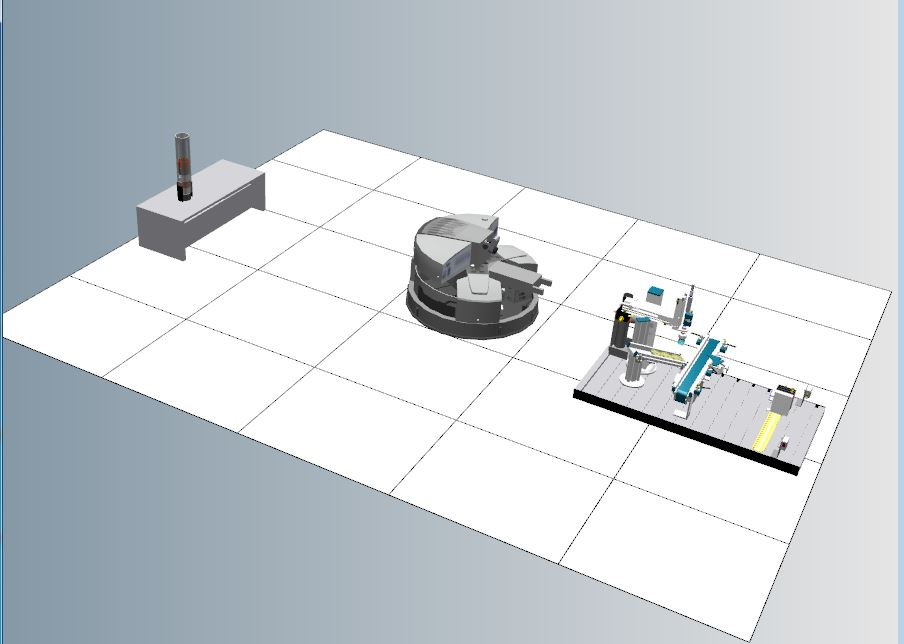
\includegraphics[height=6cm]{MPSDemo.jpg}
  \end{minipage}
} 
\quad
\subfigure[Selection of MPS workpieces]{%
  \label{fig:workpiece}%
  \begin{minipage}[b]{0.3\linewidth}
    \centering
    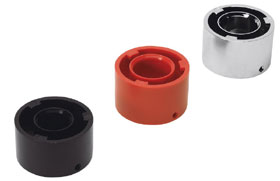
\includegraphics[height=2.5cm]{selectionofworkpieces.jpg}
    \vspace*{2cm}
  \end{minipage}
}
\caption{The challenge scenario and used workpieces}
\label{fig:mps-challenge}
\end{figure}

One robot will be required to use any gripping device to handle a
workpiece. The challenge will be to
\begin{enumerate}
\item receive one workpiece from a shelf
\item approach a "Pick \& Place" station and hand over the workpiece
\item approach the backside of this station
\item wait to receive the completed workpiece
\item transport it to one empty shelf spot and unmount it.
\end{enumerate}

\hskip-\parindent Teams may add markers of any kind to the MPS station
and shelf to support their approach. These markers have to be
removable residue-free and mounted/unmounted in a reasonable short
amount of time before each test run.

Each team has a ten minute window to conduct a test run with field
exclusivity. Once they choose to begin, they have three minutes to
complete the challenge.  Each step will be awarded with points. If all
points are completed in time, the fastest time wins.

The installation will be available throughout the whole time of the
tournament. Festo will provide one standardized gripper per team over
the course of a tournament. Custom constructions are welcome.

\paragraph{Workpiece.~}
The workpieces are round objects with a diameter of
\SI{40}{\milli\metre} and are of red, black, or silver color. They are
made of plastic, cf. \reffig{fig:workpiece}.

\paragraph{MPS station}
The MPS station is mounted on a rectangular profile plate of size
\SI{350}{\milli\metre} $\times$ \SI{700}{\milli\metre} with a height
of \SI{30}{\milli\metre}. The transfer point has a height (from
ground) of \SI{148.165}{\milli\metre}. 
% What's this?
%Handover point (centered): 
%\item From Bottom: \SI{375}{\milli\metre}
%\item From Top: \SI{325}{\milli\metre}
%\item Space between guides(center point as middle): \SI{450}{\milli\metre} diameter
%\item Height:  minimum height.
%\end{itemize}

\begin{figure}[h]
\centering
\subfigure[Overview Pick \& Place]{%
  \label{fig:mps-overview}%
  \begin{minipage}[b]{0.45\linewidth}
    \centering
    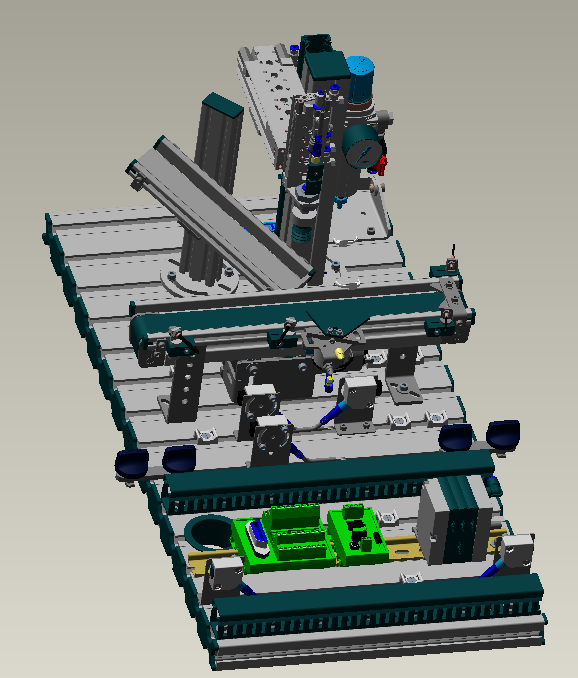
\includegraphics[height=7cm]{mps_overview.png}
  \end{minipage}
} 
\quad
\subfigure[Interface point height]{%
  \label{fig:mps-docking}%
  \begin{minipage}[b]{0.45\linewidth}
    \centering
    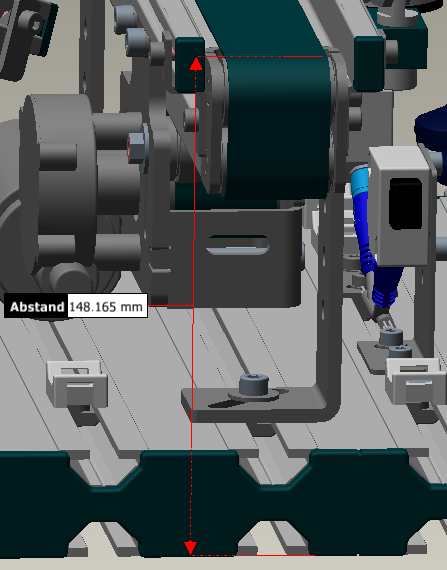
\includegraphics[height=7cm]{mps_docking.png}
  \end{minipage}
}
\caption{The MPS station in detail}
\label{fig:mps-station}
\end{figure}

\paragraph{Free challenge.~}
Each team will be given 5 minutes to showcase their robot team, e.g.
show some new robotics developments. This may involve any task as long
as it is performed with at most three Robotino robots within the
competition area. For the time of the free challenge, any software or
hardware modification is allowed, even though otherwise disallowed in
the regular competition. This may be used to showcase ideas for future
developments of the league and to highlight particular advances in the
system of the presenting team.

The team leaders of non-presenting team will judge the performance and
rate it with points between 0--10.  The team with the most sum of
points will win this challenge. The other teams are ranked in
decreasing point order.

\paragraph{Conducting the Challenges.~}
The technical challenges are conducted in the following way. The team
leader of each participating team agree on a date and time during the
tournament for the Technical Challenge in their first team leader
Meeting. For each type of challenge, a time slot is assigned in which
teams can participate once in the challenge. Each team can register
for any of the challenges. All team leaders have to be present at the
time of the challenge to judge the other teams. The OC is responsible
to conduct the Technical Challenge and can appoint team leaders to
support in conducting the challenges. Each challenge will have a
separate ranking. In each ranking, the team on the last rank will
receive 0 points, the last-but-one ranked team will receive 1 point
etc. The points for each ranking will be added and the team with the
most points accrued over all challenges will be awarded with the
Logistic Leagues Technical Challenge Award.


\section{The Robotino System}
\label{sec:robotino}

All participants have to design their competition Robotinos within the
following specifications. For a detailed technical description of the
basic hardware, refer to the Appendix~\ref{sec:engref}.

Any kind of sensors can be changed or added to the Robotino platform.
However, it is not possible to implement sensors that require
modifications outside the Robotino area (e.g. Northstar, indoor GPS).
It is furthermore strictly forbidden to implement any kind of RFID
device into the Robotino. There must be no changes to the controller
or mechanical system. The pushing device is defined as a passive,
non-mechanical load handling attachment. The robots peripherals must
not exceed the maximum total height of \SI{0.7}{\metre}. Additional
hardware (sensors, computing equipment, etc.) must be within a
diameter of \SI{0.65}{\metre} centered at the robot's rotational
center. Additional hardware may only occupy up to $25\%$ of this
additional \SI{0.15}{\centi\metre} wide ring around the robot.  The
only additional actuator allowed is one pushing device for pucks which
can be the original or a modified one. It however must not exceed the
following outside dimensions (including possibly added sensors):
\SI{0.25 x 0.15 x 0.05}{\metre} (width $\times$ depth $\times$
height). The puck must be visible from above while inside the pushing
device.

It is allowed to install additional computing power on the
\Robotino. This may either be in form of a notebook/laptop device or
any other computing device that suits the size requirement of the
\Robotino{} competition system. Furthermore, it is allowed to
communicate with an additional computing device off-field. This device
may be used for team coordination and/or other purposes. However,
communication among the robots and the off-field device is not
guaranteed during the competition.

\subsection{Markings}
\label{sec:robot-markings}
All field robots must be assigned a single unique number out of the
set $\{1, 2, 3\}$. The number must be written on the robot in one or
more places and clearly visible from all directions, e.g. printed
adhesive labels placed on top or the sides of the robot. The number
must be the same as is announced in the beacon signal to the referee
box (cf.~\refsec{sec:referee-box}).

To allow identification by the overhead camera system of the referee
box, all robots must wear unique colored labels on top of the
robot. The labels will be provided by the organizing committee. Teams
must provide appropriate mounting capabilities such that the labels
are freely and completely visible from above. The marker in 2013 will
be round labels of approximately \SI{20}{\centi\meter} in diameter
printed on paperboard.

\section{Communication}
\label{sec:communication}

Robots have to operate autonomously, that is, without any human
interference during the game. Communication among robots and to
off-board computing units is allowed only using wifi
(cf.~\refsec{sec:wifi-regulations}). Communication is not guaranteed
and may be unavailable during parts of the game. Interruptions must be
expected and are no reason to pause or abort a game, even if they
endure for long periods of the game.

\subsection{Bandwidth Allocation}
\label{sec:bandwidth}
No minimum bandwidth is guaranteed. The amount of communicated data
over the wifi connection shall not exceed
\SI[per-mode=symbol]{2}{\mega\bit\per\second}. Even though the lower
layers could provide for more bandwidth, the overall available
frequency spectrum and wifi channels have to be shared, not only
within our own league. Generally, a conservative use of bandwidth
resources is advised. Should a frequently or endured exceedance of the
bandwidth limit become known, or if the overall bandwidth limit must
be reduced due to outer circumstances, the TC can monitor the network
traffic and demand reduction in communicated data as necessary.

\subsection{Referee Box}
\label{sec:referee-box}
The referee box (refbox) is a software system that runs on a system
provided by the Organization Committee. It controls the overall game,
monitors feedback from the robots, and awards points. It is instructed
by an assisting human referee and keeps a log of all relevant game
events. The final game report will be produced by the referee
box. While we strive for a maximum of automation of this control task,
we rely on the human referee for final judgment, in particular for
border or under-specified cases, and will provide the largest set of
override abilities feasible.

The refbox is the single point of instruction for robots during the
game. After game setup has finished, game state information and orders
are announced by the refbox. Commands must be acknowledged. In certain
situations (for example during the exploration phase) for successful
and true communication with the refbox points are awarded. The aim is
to reduce human interference year by year to a minimum as to exhibit
the widest autonomy during the game possible. Ultimately, the refbox
should be able to fully control the game by itself, transforming all
participants, team members, and visitors alike into pure spectators of
the game, sometimes providing maintenance and crisis intervention when
necessary.

The communication from the refbox to the robot is a datagram-oriented
broadcast protocol based on Google protocol buffers\footnote{Available
  at \url{https://code.google.com/p/protobuf/}} (protobuf). The
protocol definition and technical parameters are described in detail
in the RoboCup Logistics League Referee Box Integrator's Manual.

\subsection{Remote Control}
\label{sec:remote-control}
Remote operation or instruction of any kind of the robots is forbidden
at all times during a game. The only allowed interaction is for the
start-up (cf.~\refsec{sec:game-start}). Any failure to comply with
this rule will lead to immediate disqualification of the infringing
team.

\subsection{Monitoring}
\label{sec:monitoring}
\emph{Passive} monitoring, i.e. receive-only communication from a base
station of the robots' performance is allowed. However, the overall
bandwidth limit may not be exceeded.
%, this includes in particular, but
%is not limited to, images and other raw data.
If the referee has any reason to belief that a monitoring application
might be used for instruction, he can demand the shutdown of the
monitoring software (also refer to previous section on Remote
Control).

\subsection{Inter-robot Communication}
\label{sec:inter-robot-comm}
Robots currently active on the field can freely exchange any
information that supports a coordinated team play. Robots not actively
participating in the game, for example because they have been
irrevocably removed from the current game, may not communicate with
the other robots. It is forbidden to communicate with any sensors that
are not physically attached to the robot, including, for example, but
not limited to a camera aside the field. Likewise any off-robot
actuator is forbidden.

\subsection{Communication Eavesdropping and Interference}
\label{sec:comm-tampering}
% This might sound harsh, but it's based on lessons learned in
% numerous years of RoboCup, you wouldn't believe what some teams will
% do... :-/
Communication of another team may neither be eavesdropped on nor be
interfered with. Teams not currently active shall disconnect from the
field access points.

Monitoring of bandwidth used or of possible misbehavior may only be
performed by members of the TC or an appointed delegate.
% can add this, need to be clear that this must be done using a team
% leader majority vote and not just any team leader
% or by a person appointed by the team leaders.
Any indication of misbehavior will be discussed by the team leader
convention and may result in penalties or disqualification from the
tournament.


%Each robot has to operate autonomously. The communication between the
%robot and the device responsible for the Start/Stop command, as well
%as all communication amongst the robots has to be realized using the
%Wi-Fi connection. The program controlling the robot has to be executed
%locally by the robot itself. % It is strictly forbidden to use any kind
%% of external server acting as command point.
%\begin{rulechange}
%  The robots will receive their commands from the Referee-Box as
%  specified in the referee box protocol. Further, communication to one
%  dedicated off-board computing device is allowed. However, wifi
%  communication should not taken for granted during competition by the
%  participating teams. 
%\end{rulechange}
%The robots are allowed to share information with other devices, but
%must receive nothing else but the start, pause and stop command
%from units other than the 2 fellow robots. This specifically excludes:
%Usage of processed image data created outside of the robots A central
%communication that requires a device other than the three Robotinos A
%permanently established connection between the command device and the
%Robotinos.

\subsection{Wifi Regulations}
\label{sec:wifi-regulations}
In order to provide the optimal possible solution for wireless
communication during the event, all teams are required to use the
\SI{5}{\giga\hertz} wifi equipment. They are furthermore required to
connect their Robotinos wifi unit to the access point provided. All
teams can also rely on wifi clients supplied by Festo but are not
required to. A detailed description concerning the infrastructure can
be found in Appendix~\ref{sec:wifi-equipment}.

% Please refer to Sect.~\ref{sec:radio-interference} for further details.

%%%%%%%%%%%%%%%%%%%%%%%%%%%%%%%%%%%%%%%%%%%%%%%%%%%%%%%%%%%%%%%%%%%%%%%%%%%%%
%%%


%%%%%%%%%%%%%%%%%%%%%%%%%%%%%%%%%%%%%%%%%%%%%%%%%%%%%%%%%%%%%%%%%%%%%%%%%%%%%
%%%

% \section{Development / Vision}

% This section is meant to enable discussions and support investment
% decisions for future soft- and hardware acquisitions.

% \subsection{Short term ideas}

% These are ideas that could still be incorporated into the rulebook of
% Istanbul 2011. 

% \subsubsection{Scripted, dynamic obstacles}

% On the way to fully dynamic obstacles this iteration implies a fully
% scripted administration controlled Robotino that follows implicit
% movement rules that are known to all participants.

% \subsection{Midterm planning}
% Additions and alterations for future iterations of this competition


% \subsubsection{Various Production programs}
% A part from the three-staged production process, various goods with
% different work orders and specifications (e.g. top speed, delivery
% strategies...) could be part of the challenge. This addition seems to
% be heavily dependent on Sect.~\ref{sec:supp-flow}.

% \subsubsection{Various order strategies}
% A delivery could consist of more than one final product, it could be
% required to deliver a batch of products, maybe within a certain time
% span, to complete the loading and receive extra points. Also, the
% different delivery gates could obtain a predefined shipping list, for
% example gate 1 requiring 2 Products, 2 M2 and 1 M1, maybe in the
% correct order to enable FIFO, LIFO or other delivery strategies.

% \subsubsection{Simulation league}

% Since there is only the annually world championship and maybe a
% regional preregistration, a simulation platform could be provided,
% where the software framework of teams can be used to compete with
% other teams. Additionally a branch of simulation could be created that
% focuses on the simulation of many AGV and a huge production area in
% order to compete on scalability.

% \subsubsection{Introducing a supportive flow of information}
% \label{sec:supp-flow}

% As the current task only deals with the material stream, it is heavily
% limited to a simple static task. In order to enable a flow of
% information that transports complex orders, a combined effort should
% focus on implementing a data interface that can be used by all teams
% today and in the future. As this would be a giant leap towards the
% industrial application, a general discussion and a lot of effort has
% to be invested into this issue.


% \subsection{Long term Vision}
% Ideas, dreams and ideology that inspire the future development.

% \subsubsection{Complex production machines}
% As there are more ways to interact with a machine than mounting and
% dismounting a loading carrier, it is possible to develop new machine
% types that look different and are completely different to handle.

% \subsubsection{Collaborative Production}
% Teams could be required to cooperate with another team to enable a
% combined supply chain. 

% \subsubsection{Opponent controlled dynamic obstacles}
% No scripted obstacle can truly represent challenges of the industrial
% application. In the long run, an opposing team has to be reinserted
% that is allowed and requested to anticipate the logistic processes in
% real time in order to create worst case scenarios for the teams.

% \subsubsection{Interfacing ERP / SCM}
% The interface used to present orders could be back ended with software
% from real business applications like ERP, PPS, WHM and SCM.

% \subsubsection{JIS / JIT implementation}
% With complex production processes and several other achievements and
% upgrades it could be useful to implement JIS and JIT tasks and
% procedures into the LL, requiring delivery strategies like LIFO, FIFO
% and certain time windows.

%%%%%%%%%%%%%%%%%%%%%%%%%%%%%%%%%%%%%%%%%%%%%%%%%%%%%%%%%%%%%%%%%%%%%%%
%%% 

\begin{appendix}
\newpage

\section{Engineering Reference}
\label{sec:engref}
\subsection{The Mobile Robot System Robotino 3}
The mobile robot system Robotino is a platform with open mechanical
and electrical interfaces for the integration of additional devices
like sensors or motors. By default power is supplied via two
exchangeable \SI{12}{\volt} lead gel batteries which permit a running
time of up to two hours. Robotino is driven by 3 independent,
omni-directional drive units. They are mounted at an angle of
\ang{120} to each other. The three omni-directional drive units of
Robotino defines it as being holonomic, meaning that the controllable
degrees of freedom equals the total degrees of freedom of the
robot. The drive units are integrated in a sturdy, laser welded steel
chassis. The chassis is protected by a rubber bumper with integrated
switching sensor.

\subsubsection{Robot Dimensions (w/o extension tower)}
\label{apx:sec:robot}
\begin{itemize}
\item \textbf{Diameter:} \SI{450}{\milli\metre}
\item \textbf{Height including housing:} \SI{290}{\milli\metre}
\item \textbf{Overall weight:} approx. \SI{22.5}{\kilogram}
\item \textbf{Maximal payload:} about \SI{30}{\kilogram}
 \end{itemize}

\subsubsection{Drive Unit}
\begin{itemize}
\item \textbf{3$\times$ omni-directional wheels:} \SI{120}{\milli\metre}
\item \textbf{Fed by DC three motors:} \SI{3600}{rpm}
\item \textbf{Gear transmission ratio 32:1} \SI{22.5}{\kilogram}
 \end{itemize}

\begin{figure}[h]
\centering
\subfigure[Festo Robotino 2]{%
  \label{fig:robotino-2}%
  \begin{minipage}[b]{0.3\linewidth}
    \centering 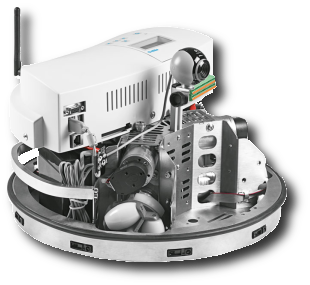
\includegraphics[height=3.5cm]{figures/robotino-shadow}
  \end{minipage}
} 
\quad
\subfigure[Festo Robotino 3]{%
  \label{fig:robotino-3}%
  \begin{minipage}[b]{0.3\linewidth}
    \centering
    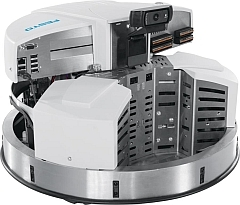
\includegraphics[height=3.5cm]{Robotino3.jpg}
  \end{minipage}
}
\caption{Robotino 2 and Robotino 3 without extension tower}
\label{fig:robotinos}
\end{figure}

\hskip-\parindent The motor speed will be controlled via a PID
controller implemented on a Atmel microprocessor of the controller
board of Robotino.

\subsubsection{Sensors}
Robotino is equipped with 9 vertical mounted infrared distance
measuring sensors which are mounted in the chassis at an angle of
\ang{40} to one another. Robotino can scrutinize all surrounding areas
for objects with these sensors.  Each of the sensors can be queried
individually via the controller board. Obstacles can thus be avoided,
clearances can be maintained and bearings can be taken on a selected
target. The sensors are capable of accurate or relative distance
measurements to objects at distances of \SI{4}{\centi\metre} to
\SI{30}{\centi\metre}. Sensor connection is especially simple
including just one analogue output signal and supply power. The
sensors' evaluation electronics determines distance and read it out as
an analogue signal.  The anti-collision sensor is comprised of a
switching strip which is secured around the entire circumference of
the chassis. A reliably recognizable signal is thus transmitted to the
controller unit.  Collisions with objects at any point on the housing
are detected and, for example, Robotino is brought to a
standstill. The inductive proximity sensor is supplied as an
additional component. It serves to detect metallic objects on the
floor.

The default webcam camera is plugged in via USB and is capable of full
HD 1080p video with auto light correction and two built in microphones
for stereo sound with noise-cancelling

\subsubsection{Controller Board}
Robotino is powered by an exchangeable Embedded PC - COM Express
layout combined with a custom made sensor board.

\paragraph{Embedded PC according to COM Express specification}
\begin{itemize}
\item Embedded Intel Core i5, 2.4 GHz, Dual-Core
\item 8 GB RAM
\item 64 GB SSD (exchangeable) 
\item Operating system: Linux Ubuntu 12.04 (64-bit)
\end{itemize}

\paragraph{Embedded PC interfaces}
\begin{itemize}
\item 1 $\times$ Ethernet
\item 6 $\times$ USB 2.0
\item 2 $\times$ PCI Express expansion slot
\item Wireless LAN according to 802.11b/g, client or access point mode
\item 2 $\times$  RS232
\item 1 $\times$ Parallel port and 1 $\times$ VGA port
\item Wireless LAN Access Point following the standards 802.11/b/g.
\item The access point supports client mode, optional WPA2 encryption.
\end{itemize}

\paragraph{Motor control}
\begin{itemize}
\item microcontroller with 32-bit microprocessor and separated
  Ethernet interface
\item Including 1 $\times$ additional motor output and encoder
  connector
\item 8 $\times$ analog inputs from 0 V to 10 V (50 Hz)
\item 8 $\times$ digital inputs/outputs with 24 V, short circuit proof
  and overload protected
\end{itemize}

\subsubsection{Power supply}
\begin{itemize}
\item 2 $\times$ 12 V lead-fleece rechargeable batteries with 9.5 Ah
  capacity each
\item Operating time(default batteries): up to 4 hours
\item Power supply for additional components: 13 x 24 V, 13 x GND
\item Internal charger for lead-gel and NiMH rechargeable batteries
\item 24 V power supply for charging batteries
\end{itemize}

\subsubsection{Software}
Pre-installed is Ubuntu Linux 12.04 LTS operating system. The main
part of the controller is the Robotino server, a real time Linux
application. It controls the drive units and provides interfaces to
communicate with external PC applications via wifi. Also provided: API
2.0 with libraries which allow you to create applications for Robotino
in numerous programming languages:

\begin{itemize}
\item C++ and C 
\item C\# 
\item .net and JAVA 
\item MatLab and Simulink
\item Labview
\item Robot Operating System (ROS)
\item Microsoft Robotics Developer Studio
\end{itemize}

You may find a lot of examples concerning using the different API's in
the public OpenRobotino forum at \url{http://www.openrobotino.org}.

\paragraph{Webinterface}
HTML5-based user interface provided by webserver running on Embedded
PC for setup and configuration using SmartPhone, Tablet or PC/Notebook
User interface supporting program management, manual control, network
setup, status display and options Help system: online manual for
getting started, details on all components and introduction into
programming

\paragraph{Robotino View} 
For a quick start or Hardware testing there is proprietary drag and
drop Software Robotino View. Graphical programming environment for
external PC running on Windows XP, Vista, Windows 7 or Windows 8.

\begin{itemize}
\item Main program using sequential function chart according to IEC 61131
\item Reusable subprograms based on function blocks
\item Library for function blocks and devices
\item Global variables for communication between subprograms
\item Program interpreter to run programs on Embedded PC autonomously
\end{itemize}

\hskip-\parindent Additional information as well as accessories can be
obtained through\\
\url{http://www.robocup-logistics.org/festo-robotino-3}\\
(redirects to Festo page).

\subsection{Robotino 2.0 (phase-out model)}
The mobile robot system Robotino is a platform with an open
mechanical interface for the integration of additional mechanical
devices and an open electrical interface to integrate easily
additional sensors or motors of devices. Power is supplied via two
\SI{12}{\volt} lead gel batteries which permit a running time of up to
two hours.  The scope of delivery likewise includes a charging
device. Robotino is driven by 3 independent, omni-directional drive
units. They are mounted at an angle of \ang{120} to each other. The
three omni-directional drive units of Robotino, defines the robot as
being holonomic, meaning that the controllable degrees of freedom
equals the total degrees of freedom of the robot. The drive units are
integrated in a sturdy, laser welded steel chassis. The chassis is
protected by a rubber bumper with integrated switching sensor.

\subsubsection{Robot Dimensions}\label{apx:sec:robot}
\begin{itemize}
\item \textbf{Diameter:} \SI{370}{\milli\metre}
\item \textbf{Height including housing:} \SI{210}{\milli\metre}
\item \textbf{Overall weight:} approx. \SI{11}{\kilogram}
\item \textbf{Maximal payload:} about \SI{6}{\kilogram}
\end{itemize}

\subsubsection{Drive Unit}
Each of the 3 drive units consists of the following components: DC
Dunker motor with nominal speed of \SI{3600}{rpm} and nominal torque
of \SI{3.8}{\newton\centi\metre}. Integrated planetary gear unit with
a gear ratio of 4:1. Omni-directional wheels of diameter of
\SI{80}{\milli\metre}. Toothed belt with gear wheels providing a
transmission ratio of 4:1. Altogether this provides a gear
transmission ratio of 16:1. Incremental encoder with a resolution of
2048 increments per motor rotation. The motor and gear arrangement is
shown in Figure~\ref{fig:driveunit}.

The motor speed will be controlled via a PID controller implemented on
a Atmel microprocessor of the controller board of Robotino.

\subsubsection{Sensors}
Robotino is equipped with 9 infrared distance measuring sensors which
are mounted in the chassis at an angle of \ang{40} to one
another. Robotino can scrutinize all surrounding areas for objects
with these sensors.  Each of the sensors can be queried individually
via the controller board. Obstacles can thus be avoided, clearances
can be maintained and bearings can be taken on a selected target. The
sensors are capable of accurate or relative distance measurements to
objects at distances of \SI{4}{\centi\metre} to
\SI{30}{\centi\metre}. Sensor connection is especially simple
including just one analogue output signal and supply power. The
sensors' evaluation electronics determines distance and read it out as
an analogue signal.  The anti-collision sensor is comprised of a
switching strip which is secured around the entire circumference of
the chassis. A reliably recognizable signal is thus transmitted to the
controller unit.  Collisions with objects at any point on the housing
are detected and, for example, Robotino is brought to a
standstill. The inductive proximity sensor is supplied as an
additional component. It serves to detect metallic objects on the
floor.

The inductive proximity sensor must be attached to the mounting
furnished for this purpose, and must be connected to the I/O
interface.  The output voltage is \SI{0}{\volt} to \SI{10}{\volt}. The
sensing range is \SI{0}{\milli\metre} to \SI{6}{\milli\metre}. Path
tracking can also be implemented with the two included diffuse
sensors.  Flexible fiber optic cables are connected to a fiber-optics
unit which works with visible red light. Reflected light is
detected. Different surfaces and colors produce different degrees of
reflection. However, gradual differences in reflected light cannot be
detected. The sensors must be attached to the mountings furnished for
this purpose, and must be connected to the I/O interface.

Robotino is equipped with a color webcam. The webcam is equipped with
a USB interface. Also, there will be integrated a digital Gyroscope
providing a high accuracy of the odometry in the virtual factory.

\subsubsection{Controller Board – 2010 Revision}

\begin{figure}[h]
\centering
\subfigure[Drive unit with motor (1), encoder (2), omni-directional wheel (3)]{%
  \label{fig:driveunit}%
  \begin{minipage}[b]{0.4\linewidth}
    \centering 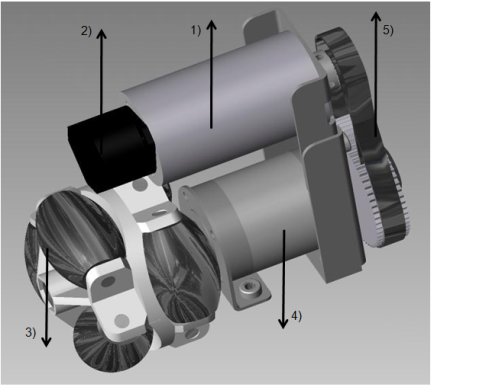
\includegraphics{driveunit.png}
  \end{minipage}
} 
\quad
\subfigure[Festo Robotino 2 inside view]{%
  \label{fig:robotino-2-board}%
  \begin{minipage}[b]{0.45\linewidth}
    \centering
    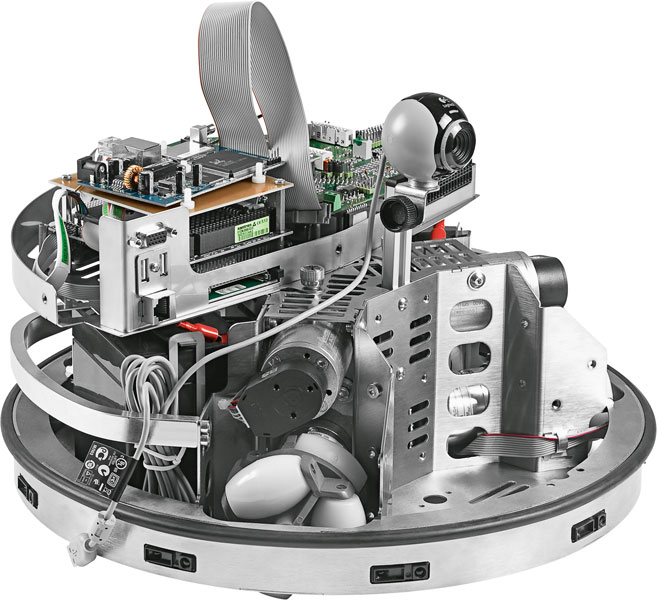
\includegraphics[height=5.5cm]{RobotinoOpen.jpg}
  \end{minipage}
}
\caption{Robotino 2 internals}
\label{fig:robotino-2-guts}
\end{figure}

The controller housing is connected to the wiring in the chassis via
one plug-in. Thus you can easily take off the controller housing and
you have direct access to the mechanical system. The controller system
of Robotino is divided into two parts – an embedded PC and a
micro-controller interface card: The Controller of Robotino consists of
an embedded PC and a micro-controller interface board. The main
controller is the embedded PC 104 plus controller with the 500 MHz
processor AMD LX800. The PC has a SDRAM of 128 MB and is provided with
a 1 GB flash card. There are numerous communication interfaces on
board:

\begin{itemize}
\item 2 $\times$ \SI[per-mode=symbol]{100}{\mega\bit\per\second} Ethernet
\item 2 $\times$ external USB, 1 $\times$ on-board USB-connector
\item 2 $\times$  RS232
\item 1 $\times$ Parallel port and 1 $\times$ VGA port
\item Wireless LAN Access Point following the standards 802.11/b/g.
\item The access point can be switched into a client mode.  As an
  option you may use WPA2-coding.
\end{itemize}

\subsubsection{Software}
Pre-installed is an Ubuntu Linux operating system with real time kernel
running on the embedded PC 104. The main part of the controller is the
Robotino server, a real time Linux application. It controls the drive
units and provides interfaces to communicate with external PC
applications via wifi. There is an API with libraries which allow you
to create applications for Robotino in numerous programming languages:

\begin{itemize}
\item C++ and C 
\item C\# 
\item .net and JAVA 
\item MatLab and Simulink
\item Labview
\end{itemize}

\hskip-\parindent You may find a lot of examples concerning using the
different API's in the public OpenRobotino forum at
\url{http://www.openrobotino.org}.

\paragraph{Robotino View} 

Robotino View is a graphical programming language with numerous
prepared function blocks you can easily connect via input and output
parameters to establish more complicated function diagrams. You can use
these function diagrams as subprograms for more complex programming
sequences. To build up general programming sequences Robotino View
follows the international standard IEC 61131-3. You may run Robotino
View on an external PC and Robotino View communicates directly with
the Robotino Server on the PC 104 via wifi in order to control the
robot system. The function blocks receive a direct feedback of the
hardware components such that you can live interact with the robot
system. On the other hand you can download Robotino View programs into
the PC 104 in order to run the applications completely autonomously.
There is a well defined interface to develop own function blocks in C++
or Lua.

\paragraph{Image Processing}

Depending on the Robotino version it might happen that the standard web
camera only provides image data by JPEG compression. This is very
useful if you run your image processing on the PC and exchange the data
via wifi. However, if you would like to run your image processing
algorithms on the Robotino controller then the processor is not
powerful enough in order to pack and to unpack the image data in a
reasonable time. Thus we recommend for running image processing
algorithms on the Robotino controller to use a camera without JPEG
compression, e.g. use the low cost Logitech web camera C250.

\subsection{Machines}
\label{abx:sec:machine}

\begin{figure}[h]
\centering
\subfigure[Ranges and dimensions of a signal]{%
  \label{apx:fig:machinemeasures}%
  \begin{minipage}[b]{0.45\linewidth}
    \centering 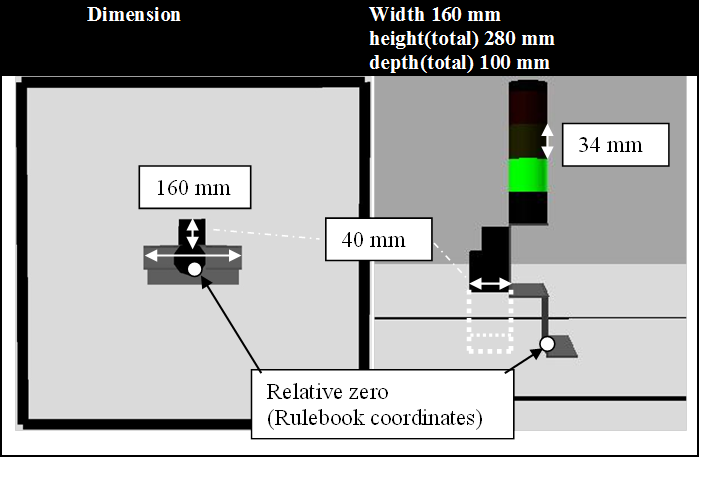
\includegraphics[width=\textwidth]{machine_measures.png}
  \end{minipage}
}
\quad
\subfigure[Ranges and dimensions of the supporting brackets]{%
  \label{apx:fig:brackets}%
  \begin{minipage}[b]{0.45\linewidth}
    \centering
    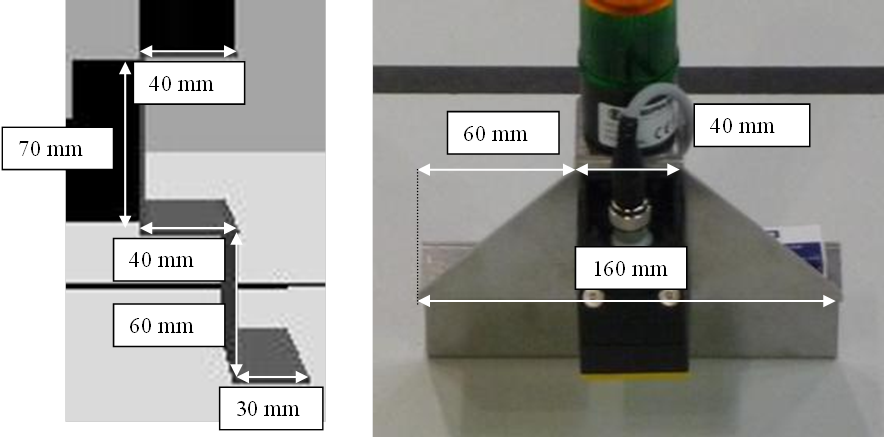
\includegraphics[width=\textwidth]{bracket.png}
  \end{minipage}
}
\caption{Machine Details}
\label{fig:machine-details}
\end{figure}

\subsubsection{Signal}
\begin{table}[H]
  \centering
  \mytable{\begin{tabularx}{\linewidth}{l|X}
      \hline
      Dimension \&	diameter&	\SI{36}{\milli\metre} \\
      height(total)		 	&	\SI{147}{\milli\metre} \\
      Segment height 			&	\SI{34}{\milli\metre},
      including \SI{5}{\milli\metre} unlighted border \\
      Lifespan				&	max. \SI{50.000}{\hour} \\
      Connector				&	Bottom, \SI{2}{\metre} supplied 
      Compatible to the I/O-Terminal of MPS(r) units. \\
      Safety					&	IP65 \\
      Voltage					&	\SI{24}{\volt} \\
      Current					&	3 $\times$ \SI{40}{\milli\ampere} \\
      Kind of current			&	DC \\
      Operating mode			&	\SIrange{-20}{+50}{\degreeCelsius} \\
      Signal type				&	Static LED \\
      Signal					&	Ultra-bright LED\\
      Source					&	Festo \# 549843 \\
%      \hline
    \end{tabularx}}
  \caption{Technical specification of the signal}
  \label{apx:tab:signalproperties}
\end{table}

\subsubsection{RFID device}

\begin{table}[H]
  \centering
  \mytable{\begin{tabularx}{1\linewidth}{l|X}
      \hline
      Technical data of the read/write head		&	Housing rectangular \\
      Housing and working dimensions 				&
      \SI{40x40}{\milli\metre}  with the centered RFID
      tag. \\
      Housing height
      & \SI{65}{\milli\metre} \\ 
      Operating voltage							&	DC \\
      Housing material Plastic					& 	PBT-GF30-V0, black \\
      Material active face Plastic				& 	PA6-GF30, yellow \\
      Operating voltage
      & 	\SIrange{10}{30}{\volt.DC} \\
      DC rated operational current				& 	$\le$ \SI{80}{\milli\ampere} \\
      Data transfer								& 	inductance coupling \\
      Working frequency							& 	\SI{13.56}{\mega\hertz} \\
      Radio communication and protocol standards	&	ISO 15693 \\
      Read/write distance							&	max. \SI{115}{\milli\metre} \\
      Output function								&	4-wire, read/write \\
      Electrical connection 						&	Connectors M12 $\times$ 1 \\
       Vibration resistance						&	\SI{55}{\hertz} (\SI{1} {\milli\metre}) \\
       Shock resistance							&	\SI{30}{\gram} (\SI{11}{ \milli\second}) \\
       Protection class							&	IP67 \\
       Operating voltage display					& 	LED green \\
% %      \hline
    \end{tabularx}}
  \caption{Technical specification of the RFID device}
  \label{apx:tab:rfidproperties}
\end{table}

\subsubsection{Wifi equipment}
\label{sec:wifi-equipment}
\begin{table}[H]
  \centering
  \mytable{
    \begin{tabularx}{1\linewidth}{l|X}
      \hline
      Festo AP		&	LANCOM L-322agn \\
      Transfer rate		&	Up to \SI{108}{\mega\bit\per\second} \\
      Data link protocol	&	802.11 a/g/n \\
      Frequency			&	\SI{5.0}{\giga\hertz} \\
      IP-distribution		&	172.26.200.xxx for LAN clients(DHCP) \\
      &	172.26.101.xxx for the Robotino devices \\
      &	172.26.1.xxx for Robotinos \\
      Subnet Mask			&	255.255.0.0 \\
      Encryption			&	Unsecured \\
      SSID				&	Separated for both teams:\\
      &	RobotinoEvent.1 \\
      & RobotinoEvent.2 \\
      Festo Clients		&	3COM WL-560 \\
      Power Supply		&	Clients: \SI{12}{\volt}, \SI{1}{\ampere},\\
      & 	Most Laptops cannot power them \\
      & 	via USB! \\
      Connector			&	Ethernet \\
      
%      \hline
    \end{tabularx} }
    \caption{Technical specification of the wifi equipment}
	\label{apx:tab:wifi}
\end{table}

\subsubsection{Data carrier}
\label{sec:data-carrier}
\begin{table}[H]
  \centering
  \mytable{
    \begin{tabularx}{\linewidth}{l|X}
      \hline
      Dimension									&	\diameter  \SI{20}{\milli\metre} \\
      Height										&	\SI{2.5}{\milli\metre} \\
      Data transfer								&	inductance coupling \\
      Working frequency							&	\SI{13.56}{\mega\hertz} \\
      Memory 										&	read/write \\	
      Memory type									&	EEPROM \\
      Memory size									&	\SI{128}{\byte} \\
      Freely usable memory						&	\SI{112}{\byte} \\
      Number of read operations					&	unlimited \\
      Number of write operations					&	105 \\
      Typical read time							&	\SI{2}{\milli\second\per\byte} \\
      Typical write time							&	\SI{3}{\milli\second\per\byte} \\
      Radio communication and protocol standards	&	ISO 15693 \\
      
      % \hline
    \end{tabularx}}
  \caption{Technical specification of the data carrier}
  \label{apx:tab:datacarrier}
\end{table}

\printbibliography

\end{appendix}
\end{document}
